\documentclass[12pt]{article}

\author{Matthew D. Cocci}
\title{Econometrics}
\date{\today}

%% Formatting & Spacing %%%%%%%%%%%%%%%%%%%%%%%%%%%%%%%%%%%%

%\usepackage[top=1in, bottom=1in, left=1in, right=1in]{geometry} % most detailed page formatting control
\usepackage{fullpage} % Simpler than using the geometry package; std effect
\usepackage{setspace}
%\onehalfspacing
\usepackage{microtype}

%% Formatting %%%%%%%%%%%%%%%%%%%%%%%%%%%%%%%%%%%%%%%%%%%%%

%\usepackage[margin=1in]{geometry}
    %   Adjust the margins with geometry package
%\usepackage{pdflscape}
    %   Allows landscape pages
%\usepackage{layout}
    %   Allows plotting of picture of formatting



%% Header %%%%%%%%%%%%%%%%%%%%%%%%%%%%%%%%%%%%%%%%%%%%%%%%%

%\usepackage{fancyhdr}
%\pagestyle{fancy}
%\lhead{}
%\rhead{}
%\chead{}
%\setlength{\headheight}{15.2pt}
    %   Make the header bigger to avoid overlap

%\fancyhf{}
    %   Erase header settings

%\renewcommand{\headrulewidth}{0.3pt}
    %   Width of the line

%\setlength{\headsep}{0.2in}
    %   Distance from line to text


%% Mathematics Related %%%%%%%%%%%%%%%%%%%%%%%%%%%%%%%%%%%

\usepackage{amsmath}
\usepackage{amssymb}
\usepackage{amsfonts}
\usepackage{mathrsfs}
\usepackage{amsthm} %allows for labeling of theorems
%\numberwithin{equation}{section} % Number equations by section
\theoremstyle{plain}
\newtheorem{thm}{Theorem}[section]
\newtheorem{lem}[thm]{Lemma}
\newtheorem{prop}[thm]{Proposition}
\newtheorem{cor}[thm]{Corollary}

\theoremstyle{definition}
\newtheorem{defn}[thm]{Definition}
\newtheorem{ex}[thm]{Example}

\theoremstyle{remark}
\newtheorem*{rmk}{Remark}
\newtheorem*{note}{Note}

% Below supports left-right alignment in matrices so the negative
% signs don't look bad
\makeatletter
\renewcommand*\env@matrix[1][c]{\hskip -\arraycolsep
  \let\@ifnextchar\new@ifnextchar
  \array{*\c@MaxMatrixCols #1}}
\makeatother


%% Font Choices %%%%%%%%%%%%%%%%%%%%%%%%%%%%%%%%%%%%%%%%%

\usepackage[T1]{fontenc}
\usepackage{lmodern}
\usepackage[utf8]{inputenc}
%\usepackage{blindtext}
\usepackage{courier}


%% Figures %%%%%%%%%%%%%%%%%%%%%%%%%%%%%%%%%%%%%%%%%%%%%%

\usepackage{tikz}
\usetikzlibrary{decorations.pathreplacing}
\usepackage{graphicx}
\usepackage{subfigure}
    %   For plotting multiple figures at once
%\graphicspath{ {Directory/} }
    %   Set a directory for where to look for figures


%% Hyperlinks %%%%%%%%%%%%%%%%%%%%%%%%%%%%%%%%%%%%%%%%%%%%
\usepackage{hyperref}
\hypersetup{%
    colorlinks,
        %   This colors the links themselves, not boxes
    citecolor=black,
        %   Everything here and below changes link colors
    filecolor=black,
    linkcolor=black,
    urlcolor=black
}

%% Colors %%%%%%%%%%%%%%%%%%%%%%%%%%%%%%%%%%%%%%%%%%%%%%%

\usepackage{color}
\definecolor{codegreen}{RGB}{28,172,0}
\definecolor{codelilas}{RGB}{170,55,241}

% David4 color scheme
\definecolor{d4blue}{RGB}{100,191,255}
\definecolor{d4gray}{RGB}{175,175,175}
\definecolor{d4black}{RGB}{85,85,85}
\definecolor{d4orange}{RGB}{255,150,100}

%% Including Code %%%%%%%%%%%%%%%%%%%%%%%%%%%%%%%%%%%%%%%

\usepackage{verbatim}
    %   For including verbatim code from files, no colors
\usepackage{listings}
    %   For including code snippets written directly in this doc

\lstdefinestyle{bash}{%
  language=bash,%
  basicstyle=\footnotesize\ttfamily,%
  showstringspaces=false,%
  commentstyle=\color{gray},%
  keywordstyle=\color{blue},%
  xleftmargin=0.25in,%
  xrightmargin=0.25in
}

\lstdefinestyle{matlab}{%
  language=Matlab,%
  basicstyle=\footnotesize\ttfamily,%
  breaklines=true,%
  morekeywords={matlab2tikz},%
  keywordstyle=\color{blue},%
  morekeywords=[2]{1}, keywordstyle=[2]{\color{black}},%
  identifierstyle=\color{black},%
  stringstyle=\color{codelilas},%
  commentstyle=\color{codegreen},%
  showstringspaces=false,%
    %   Without this there will be a symbol in
    %   the places where there is a space
  numbers=left,%
  numberstyle={\tiny \color{black}},%
    %   Size of the numbers
  numbersep=9pt,%
    %   Defines how far the numbers are from the text
  emph=[1]{for,end,break,switch,case},emphstyle=[1]\color{red},%
    %   Some words to emphasise
}

\newcommand{\matlabcode}[1]{%
    \lstset{style=matlab}%
    \lstinputlisting{#1}
}
    %   For including Matlab code from .m file with colors,
    %   line numbering, etc.

%% Bibliographies %%%%%%%%%%%%%%%%%%%%%%%%%%%%%%%%%%%%

\usepackage{natbib}
    %---For bibliographies
%\setlength{\bibsep}{3pt} % Set how far apart bibentries are

%% Misc %%%%%%%%%%%%%%%%%%%%%%%%%%%%%%%%%%%%%%%%%%%%%%

\usepackage{enumitem}
    %   Has to do with enumeration
\usepackage{appendix}
%\usepackage{natbib}
    %   For bibliographies
\usepackage{pdfpages}
    %   For including whole pdf pages as a page in doc


%% User Defined %%%%%%%%%%%%%%%%%%%%%%%%%%%%%%%%%%%%%%%%%%

%\newcommand{\nameofcmd}{Text to display}
\newcommand*{\Chi}{\mbox{\large$\chi$}} %big chi
    %   Bigger Chi

% In math mode, Use this instead of \munderbar, since that changes the
% font from math to regular
\makeatletter
\def\munderbar#1{\underline{\sbox\tw@{$#1$}\dp\tw@\z@\box\tw@}}
\makeatother

% Limits
\newcommand{\limN}{\lim_{N\rightarrow\infty}}
\newcommand{\limn}{\lim_{n\rightarrow\infty}}
\newcommand{\limt}{\lim_{t\rightarrow\infty}}
\newcommand{\limT}{\lim_{T\rightarrow\infty}}
\newcommand{\limhz}{\lim_{h\rightarrow 0}}

% Misc Math
\newcommand{\Prb}{\mathrm{P}}
\newcommand{\ra}{\rightarrow}
\newcommand{\diag}{\text{diag}}
\newcommand{\ch}{\text{ch}}
\newcommand{\dom}{\text{dom}}
\newcommand{\one}{\boldsymbol{1}}

% Script
\newcommand{\sF}{\mathscr{F}}
\newcommand{\sB}{\mathscr{B}}
\newcommand{\sL}{\mathscr{L}}
\newcommand{\sM}{\mathscr{M}}
\newcommand{\sT}{\mathscr{T}}
\newcommand{\sA}{\mathscr{A}}

% Boldsymbol
\newcommand{\bsb}{\boldsymbol{b}}
\newcommand{\bshatb}{\boldsymbol{\hat{b}}}
\newcommand{\bsd}{\boldsymbol{d}}
\newcommand{\bsg}{\boldsymbol{g}}
\newcommand{\bsG}{\boldsymbol{G}}
\newcommand{\bsJ}{\boldsymbol{J}}
\newcommand{\bsh}{\boldsymbol{h}}
\newcommand{\bsS}{\boldsymbol{S}}
\newcommand{\bsu}{\boldsymbol{u}}
\newcommand{\bsx}{\boldsymbol{x}}
\newcommand{\bsX}{\boldsymbol{X}}
\newcommand{\bsy}{\boldsymbol{y}}
\newcommand{\bsY}{\boldsymbol{Y}}
\newcommand{\bstheta}{\boldsymbol{\theta}}
\newcommand{\bsmu}{\boldsymbol{\mu}}
\newcommand{\bsSigma}{\boldsymbol{\Sigma}}
\newcommand{\bshatmu}{\boldsymbol{\hat{\mu}}}
\newcommand{\bshatSigma}{\boldsymbol{\hat{\Sigma}}}

% Transposes of all the boldsymbol shit
\newcommand{\bsbp}{\boldsymbol{b'}}
\newcommand{\bshatbp}{\boldsymbol{\hat{b'}}}
\newcommand{\bsdp}{\boldsymbol{d'}}
\newcommand{\bsgp}{\boldsymbol{g'}}
\newcommand{\bsGp}{\boldsymbol{G'}}
\newcommand{\bshp}{\boldsymbol{h'}}
\newcommand{\bsSp}{\boldsymbol{S'}}
\newcommand{\bsup}{\boldsymbol{u'}}
\newcommand{\bsxp}{\boldsymbol{x'}}
\newcommand{\bsyp}{\boldsymbol{y'}}
\newcommand{\bsthetap}{\boldsymbol{\theta'}}
\newcommand{\bsmup}{\boldsymbol{\mu'}}
\newcommand{\bsSigmap}{\boldsymbol{\Sigma'}}
\newcommand{\bshatmup}{\boldsymbol{\hat{\mu'}}}
\newcommand{\bshatSigmap}{\boldsymbol{\hat{\Sigma'}}}


% Mathcal
\newcommand{\calD}{\mathcal{D}}
\newcommand{\calF}{\mathcal{F}}
\newcommand{\calG}{\mathcal{G}}

% Blackboard
\newcommand{\R}{\mathbb{R}}
\newcommand{\Rn}{\mathbb{R}^n}
\newcommand{\RN}{\mathbb{R}^N}
\newcommand{\Rk}{\mathbb{R}^n}
\newcommand{\Rnn}{\mathbb{R}^{n\times n}}
\newcommand{\C}{\mathbb{C}}
\newcommand{\Cn}{\mathbb{C}^n}
\newcommand{\Cnn}{\mathbb{C}^{n\times n}}
\newcommand{\E}{\mathbb{E}}
\newcommand{\N}{\mathbb{N}}

\DeclareMathOperator*{\argmin}{arg\;min}
\DeclareMathOperator*{\argmax}{arg\;max}
\newenvironment{rcases}
  {\left.\begin{aligned}}
  {\end{aligned}\right\rbrace}

% Redefine real and imaginary from fraktur to plain text
\newcommand{\Cov}{\operatorname{Cov}}
\newcommand{\Corr}{\operatorname{Corr}}
\newcommand{\Var}{\operatorname{Var}}
\newcommand{\asto}{\xrightarrow{a.s.}}
\newcommand{\pto}{\xrightarrow{p}}
\newcommand{\msto}{\xrightarrow{m.s.}}
\newcommand{\dto}{\xrightarrow{d}}
\newcommand{\Lpto}{\xrightarrow{L_p}}
\newcommand{\plim}{\text{plim}_{n\rightarrow\infty}}

% Redefine real and imaginary from fraktur to plain text
\renewcommand{\Re}{\operatorname{Re}}
\renewcommand{\Im}{\operatorname{Im}}

% Shorter sums: ``Sum from X to Y''
% - sumXY  is equivalent to \sum^Y_{X=1}
% - sumXYz is equivalent to \sum^Y_{X=0}
\newcommand{\sumnN}{\sum^N_{n=1}}
\newcommand{\sumin}{\sum^n_{i=1}}
\newcommand{\sumkn}{\sum^n_{k=1}}
\newcommand{\sumtT}{\sum^T_{t=1}}
\newcommand{\sumninf}{\sum^\infty_{n=1}}
\newcommand{\sumtinf}{\sum^\infty_{t=1}}
\newcommand{\sumnNz}{\sum^N_{n=0}}
\newcommand{\suminz}{\sum^n_{i=0}}
\newcommand{\sumknz}{\sum^n_{k=0}}
\newcommand{\sumtTz}{\sum^T_{t=0}}
\newcommand{\sumninfz}{\sum^\infty_{n=0}}
\newcommand{\sumtinfz}{\sum^\infty_{t=0}}


%%%%%%%%%%%%%%%%%%%%%%%%%%%%%%%%%%%%%%%%%%%%%%%%%%%%%%%%%%%%%%%%%%%%%%%%
%% BODY %%%%%%%%%%%%%%%%%%%%%%%%%%%%%%%%%%%%%%%%%%%%%%%%%%%%%%%%%%%%%%%%
%%%%%%%%%%%%%%%%%%%%%%%%%%%%%%%%%%%%%%%%%%%%%%%%%%%%%%%%%%%%%%%%%%%%%%%%

\begin{document}
\maketitle
\tableofcontents %adds it here

\clearpage

\section{Introduction}

This document aims to bring together the elements of probability,
measure theory, and stochastic calculus useful for the anlysis of
stochastic process that have particular relevance in finance and
economics.

\section{Measure Theory Foundations}

\subsection{Finite Probability Spaces}

\subsubsection{Finite Probability Spaces}

\begin{defn}{(Sample Space)}
The \emph{sample space} $\Omega=\{\omega_1,\ldots,\omega_N\}$ is the set
of all \emph{elementary} outcomes of some statistical experiment. For a
given experiment, only one $\omega \in \Omega$ can occur when we conduct
and observe that experiment.
\end{defn}
\begin{ex}
If our experiment consists of flipping a single coin, the sample space
consisting of elementary events is $\{H,T\}$. If we flip two coins, the
sample space is $\{HH,HT,TH,TT\}$.
\end{ex}
\begin{rmk}
The previous example suggests that there's some subtlety in how you
define ``elementary'' event. In the case where we flipped two coins, it
might seem like a single flip is more ``elementary.'' However, if we define
our experiment to be the flipping of two coins, the set of outcomes from
that experiment really is $\Omega=\{HH,HT,TH,TT\}$. It's an unfortunate
bit of nomenclatural confusion.

Of course, we'll fix this quite soon when we encounter \emph{product
spaces}, which resolve a lot of this subtlety. In particular, product
spaces will let us define a narrow product space like $\Omega=\{H,T\}$
and then construct a richer probability space like
$\Omega\times \Omega = \{HH,HT,TH,TT\}$ or even $\Omega^N$, building up
from relatively simples ones.
\end{rmk}

\begin{defn}{(Finite Probability Space)}
A \emph{finite probability space} is a pair $(\Omega,P)$ consisting of a
finite sample space $\Omega=\{\omega_1,\ldots,\omega_N\}$ of elementary
events together with probabilities $\{p_1,\ldots,p_N\}$ satisfying
\begin{align*}
  \sumnN p_n = 1
  \quad\text{and}\quad
  p_n \in [0,1] \quad \forall n=1,\ldots,N
\end{align*}
where $p_n$ is the probability of elementary event $\omega_n\in\Omega$
occurring.
\end{defn}

\begin{defn}{(Event)}
An \emph{event} is any subset $A\subseteq \Omega$ of the sample space.
\end{defn}
\begin{ex}
Given sample space $\Omega=\{HH,HT,TH,TT\}$ for an experiment where we
toss two coins, we might consider the event $A=\{HH,HT\}$ which is
``heads tossed first.''
\end{ex}


\begin{defn}{(Set Algebra)}
A collection $\calF$ of subsets of $\Omega$ (i.e.\ a collection of
events) is called a \emph{set algebra}, or simply \emph{algebra}, if it
satisfies the following three properties:
\begin{enumerate}
  \item $\Omega\in\calF$
  \item $A,B\in\calF \implies A\cup B\in\calF$
  \item $A\in\calF\implies A^c\in\calF$.
\end{enumerate}
\end{defn}
\begin{rmk}
This is not to be confused with a $\sigma$-algebra, which we'll see
later. A set algebra is closed only under finite unions, which is not
going to be a problem in a finite probability space. Once we move to
infinite probability spaces, we will need $\sigma$-algebras, which are
closed under \emph{infinite} unions. But more on that later.

At any rate, the reason we care about algebras is that they collect and
contain the sets---the events---to which we will assign probabilities.
Our notion of a probability will be defined for elements in this
collection, as we see in the next definition.
\end{rmk}


\begin{defn}{(Probability Measure)}
\label{defn:finitemeasure}
Given a finite probability space, define the \emph{probability measure}
on $\Omega$ as the mapping
\begin{align*}
  \Prb&: 2^\Omega \rightarrow [0,1] \\
  \Prb[A] &:= \sum_{\{n|\omega_n\in A\}} p_n
\end{align*}
In this way, we use the probabilities $\{p_1,\ldots,p_n\}$ over the
elementary events to construct the probabilites of any event
$A\subseteq \Omega$ or $A\in\calF$.

Probability measures display the following properties
\begin{enumerate}
  \item $\Prb[\omega_n]=p_n$ for $\omega_n\in\Omega$
  \item $\Prb[\emptyset] = 0$
  \item $\Prb[\Omega] = 1$
  \item $\Prb[A\cup B] = \Prb[A] + \Prb[B] - \Prb[A\cap B]$ for any
    events $A,B$.
\end{enumerate}
\end{defn}


\begin{defn}{(Random Variable)}
A \emph{random variable} on finite probability space $\Omega$ is a
function
\begin{align*}
  X: \Omega\ra \R
\end{align*}
Since it's inconvenient to deal with sets and $\omega$'s in $\Omega$
directly, we use random variables that map these elements into the real
line. But in general, we only know how to assign probabilities to
events in $\Omega$. How can assign probabiilities to random variables?
That leads us to the next definition.
\end{defn}

\begin{defn}{($\calF$-Measurable)}
A random variable $X$ is $\calF$-measurable if
\begin{align*}
  \{X=x\} :=
  X^{-1}(x) =
  \{\omega\in\Omega \; | \; X(\omega)=x\}
  \in \calF
\end{align*}
for all $x\in\R$. The idea is that Definition~\ref{defn:finitemeasure}
tells us how to assign probabilities to events or ``measure'' events in
$\calF$. To ``measure'' or assign probabilities to random variables
taking values on the real line, we need to be able to map those values
back into the events in $\calF$ that we do know how to measure.

Not surprisingly, we differentiate between algebras and say
$\calF$-measurable because random variables might be measurable with
respect to some algebras and not others.
\end{defn}

\subsubsection{Product Spaces}

\begin{defn}{(Product Space)}
Given two finite probability spaces $(\Omega,P)$ and $(\Omega',P')$,
define a new probability space called the \emph{product space}
$(\Omega\times\Omega', P \otimes P')$ as
\begin{align*}
  \Omega\times\Omega'
  &= \{(\omega,\omega') \; |\; \omega\in\Omega, \; \omega'\in\Omega'\}
  \\
  (P \otimes P')(\omega, \omega')
  &= \Prb[\omega]\cdot \Prb[\omega']
\end{align*}
\end{defn}

\begin{defn}{(Lifting Random Variables to a Product Space)}
Suppose that we have events $A\subseteq \Omega$ and
$B\subseteq \Omega'$. We want to make sure that the same events are
defined on product space $\Omega\times \Omega'$. Then we can define new
sets
\begin{align*}
  \hat{A} &:= A\times \Omega' \\
  \hat{B} &:= \Omega \times B
\end{align*}
The probabilities of these events will be exactly the same on $\Omega
\times \Omega'$ as they were on just $\Omega$ or just $\Omega'$ because
notice
\begin{align*}
  (\Prb\otimes \Prb')[\hat{A}] &= \Prb(A) \cdot \Prb'(\Omega') = \Prb(A) \cdot 1\\
  (\Prb\otimes \Prb')[\hat{B}] &= \Prb(\Omega) \cdot \Prb'(B) = 1\cdot \Prb'(B)
\end{align*}
Moreover, $\hat{A}$ and $\hat{B}$ will be independent events, which
makes sense given that they started by having nothing to do with each
other, hanging out completely on their own in $\Omega$ or $\Omega'$.
\end{defn}

\begin{defn}{(Lifting Random Variables to a Product Space)}
We can easily ``lift'' random variables on $\Omega$ or $\Omega'$ into
the new product space $\Omega\times \Omega'$. To do so, suppose that we
have random variables $X:\Omega\ra\R$ and $Y:\Omega'\ra\R$. Then define
\begin{align*}
  \forall (\omega,\omega') \in \Omega\times \Omega' \qquad
  \begin{cases}
  \hat{X}(\omega, \omega') &= X(\omega) \\
  \hat{Y}(\omega, \omega') &= Y(\omega')
  \end{cases}
\end{align*}
Then $\hat{X}$ and $\hat{Y}$ are RVs $X$ and $Y$ suitably adapted to
live on probability space $(\Omega,\Omega')$.
\end{defn}

%\section{Probability with Measure Theory}


%\begin{rmk}
%Because a $\sigma$-algebra is closed under countable unions,
%interesections, and complements, it provides a natural way to think
%about collections of elementary outcomes that we might care about. Said
%another way, the definition of a $\sigma$-algebra results gives us
%pretty much all of the sets we'd like to assign probabilities to.
%\end{rmk}

%\begin{ex}
%For an even simpler example than die rolling of something that is
%a perfectly valid $\sigma$-algebra, we
%sometimes take the power set of $\Omega$---the collection of all
%possible subsets of $\Omega$---to be our $\sigma$-algebra.  It will
%surely satisfy the necessary properties, and it happens to be very easy
%to denote.
%\end{ex}


%\subsection{Measure}

%Once we have a $\sigma$-algebra, we can pair the sample space with it's
%$\sigma$-algebra to form what's called a
%\textbf{measurable space}, which is simply the ordered pair
%$(\Omega, \mathcal{F})$.  From there, we can start assigning
%probabilities to those elements in the $\sigma$-algebra which all have
%some chance of occurring.  To do so, we will use a special
%type of function, called a measure.

%A \textbf{measure} is a function that maps sets into real numbers.
%In our case, we will define a specific type of measure, a
%\textbf{probability measure}, as a
%function that has as it's domain a $\sigma$-algebra and maps measurable
%sets in the $\sigma$-algebra into the
%real line, subject to a few conditions. More precisely, it has the
%following characteristics:
%\begin{itemize}
   %\item[i.] If $P$ is our probability measure and $\mathcal{F}$ is
      %our $\sigma$-algebra, then
	 %\[ P: \mathcal{F} \rightarrow \mathbb{R} \]
   %\item[ii.] $ P(F) \in [0,1]$ for all measurable sets
      %$F \in \mathcal{F}$. In addition, $P(\Omega) =1$.
   %\item[iii.] Our probability measure satisfies the probability axioms.
      %And if $F_i$ are all disjoint and members of the $\sigma$-algebra,
      %then
	 %\[ p( \cup F_i) = \sum P(F_i) \]
%\end{itemize}

%\paragraph{Definition} Now that we have our definition of a probability,
%I just want to define a common term more precisely.  Specifically,
%if a property is true \emph{except} for an event of probability 0,
%then we say that property holds ``almost surely.''

%\subsection{Probability Space}

%So now we have a way of assigning probabilities to any arbitrary event in our measurable space, $(\Omega, \mathcal{F})$. If we
%join the probability measure, $P$, to our measurable space, we obtain a proper \textbf{Probability Space}.  It is defined as
%the ordered triplet
%\[(\Omega, \mathcal{F}, P) \]

%\subsection{Measurable Function and Random Variables}

%One of the fundamental notions of probability is that of a random
%variable; therefore, making the definition more rigorous
%deserves some attention.

%So let's start with the notion of a \textbf{measurable} function.
%If $(\Omega_1, \mathcal{F}_1)$ and $(\Omega_2, \mathcal{F}_2)$ are two
%measurable spaces then, a function
   %\[ f: (\Omega_1, \mathcal{F}_1) \rightarrow (\Omega_2, \mathcal{F}_2)
      %\]
%is a measurable function if
   %\[ f^{-1}(B) \in \mathcal{F}_1, \;\; \forall B \in\mathcal{F}_2 \]
%In words, a function is measurable if the pre-image of an element in
%the $\sigma$-algebra of the co-domain is in the
%$\sigma$-algebra of the domain.  Simply, it preserves the structure
%between two measurable spaces, sending measurable sets
%in one measurable space to measurable sets in the other.

%Turning to probability, suppose  that we have our probability space,
%$(\Omega_1, \mathcal{F}_1, P)$, and another measurable space,
%$(\Omega_2,\mathcal{F}_2)$.  Then an
%$\mathbf{(\Omega_2, \mathcal{F}_2)}$\textbf{-valued random variable}
%is a \emph{measurable function}
%\[ X: (\Omega_1, \mathcal{F}_1) \rightarrow (\mathbb{R},
   %\mathcal{F}_2) \]

%Since $X$ is a measurable function, we know that
   %\[ X^{-1}(B) \in \mathcal{F}_1, \;\; \forall B \in \mathcal{F}_2\]
%in which case we say that $X$ is $\mathcal{F}_1$-measurable.
%To clarify further
   %\[ X^{-1}(B) = \left\{ \omega \in \Omega_1 | X(\omega)
      %\in B \right\} \]

%\paragraph{Note} Oftentimes, we'll just take the set
%$\mathcal{F}_2$ to be some properly
%defined $\sigma$-algebra on the real line, like the Borel Set
%(defined below).

%\subsection{Sigma Algebras Generated by Random Variables}

%Above, we assumed that we knew the $\sigma$-algebra for
%$\Omega_1$ already---that it was given. But we
%could just as well \emph{generate} one from some random variable $X$,
%and this generated $\sigma$-algebra could very well differ from
%$\mathcal{F}_1$.

%So let's assume that $X$ is a random variable
   %\[X: (\Omega_1,\mathcal{F}_1) \rightarrow
      %(\mathbb{R},\mathcal{F}_2).\]
%Then the $\sigma$-algebra generated by $X$, denoted by $\sigma(X)$, is
%defined as \emph{all} sets of the form
   %\[ \sigma(X) := \{ \omega \in \Omega_1 | X(\omega) \in A \}, \;\;
      %\forall \; A \subset \mathbb{R} \]
%which can be written more compactly as
   %\[\sigma(X)  = \{ X^{-1}(A) | A\subset \mathbb{R}  \} \]

%\paragraph{Definition} Finally, if $\mathcal{G}$ is a
%sub-$\sigma$-algebra of the set $\mathcal{F}$ defined above, then the
%random variable $X$ is $\mathcal{G}$-measurable if
   %\[ \sigma(X) \subset \mathcal{G} \]

%Let's give a concrete example.  Suppose $\Omega$ consists of all the
%possible combination of up and down moves in a binomial tree.  $X$ is
%a random variable denoting stock price.  Then for a set of real numbers
%representing the possible prices the stock could take on (this is
%our $A \subset \mathbb{R}$), the set $\sigma(X)$ will be the sigma
%algebra resulting from the set of all possible paths that that the
%stock could have taken to get to those prices in $A$.

%\subsection{Random Variables and Their Distributions}

%A random variable is actually quite distinct from its distribution.  Recall that a Random Variable is just a mapping from the
%sample space $\Omega$ into something more tractable, like the real line.  Therefore, we could discuss this mapping--the random variable--
%without ever considering probabilities.

%However, oftentimes we will want to discuss probabilities, but the sufficiently general definition of the random variable just given
%offers a lot of flexibility.  So much, in fact, that a random variable could have more than one distribution, as we know occurs in
%stock process which have traditional probabilities and also \emph{risk-neutral} probabilities (or \emph{pseudo-probabilities}).

%So let's define a \textbf{distribution} as a measure that assigns probabilities to the real numbers that a random variable generates
%(after being passed an element in the sample space).  The most natural distribution is the induced measure, $\mathcal{L}_X$ defined
%as follows
%\[ \mathcal{L}_X(A) := P \{ X \in A \}, \;\; A \subset \mathbb{R} \]

%Let's unpack that. If $A$ is a subset of the real line, it the random variable may or may not take on values in that subset, so we want
%a notion of probability.  Well, we can take the pre-image, $X^{-1}(A)$, and look at all those elements of the sample space that map to
%$A \subset \mathbb{R}$ under the random variable $X$.  Then, once we have elements of the sample space, we can use our traditional notion
%of the $\sigma$-algebra, $\mathcal{F}$, and the probability measure $P$ that are already defined on the probability space to assign
%the probabilities.

%Thus, we can associate probabilities with our random variable so long as there exists a distribution measure, like $\mathcal{L}_X$.
%But recall that $\mathcal{L}_X$ was not unique.  It's simply a function to assign probabilities to values that the random variable can
%take on.  We could consider other measures that also accomplish this, and that insight legitimizes the use of such things as
%\emph{risk-neutral probabilities}.

%\subsection{Lebesgue Measure and the Lebesgue Integral}

%\subsection{Introduction}

%The \textbf{Lebesgue Measure} is the standard way of assigning a measure to subsets of $n$-dimensional Euclidean space.  If we restrict
%to $\mathbb{R}$, then the Lebesgue Measure of intervals is simply the length. But rather than consider all of $\mathbb{R}$, we'll
%restrict further to \emph{Borel Sets}.

%This will allow us to construct the \emph{Lebesgue Integral}, a generalization of the Riemann Integral.

%\subsection{Borel Sets}

%The \emph{Borel $\sigma$-algebra}, denoted $\mathcal{B}(\mathbb{R})$, is the smallest $\sigma$-algebra containing (and, in a sense,
%generated by) all open intervals
%in $\mathbb{R}$.

%\paragraph{Examples} The following are a few samples of Borel Sets in $\mathcal{B}(\mathbb{R})$:
%\begin{itemize}
   %\item{Every open interval of the form $(a,b)$.}
   %\item{The open rays $(a,+\infty)$ and $(-\infty,b)$.}
   %\item{All unions of the form
	 %\[ B_1 \cup B_2, \;\; B_1,B_2 \in \mathcal{B}(\mathbb{R}) \]
      %}
   %\item{All complements of sets in $\mathcal{B}(\mathbb{R})$, since it's a sigma algebra. Note that this implies all \emph{closed}
      %intervals in $\mathbb{R}$ are Borel Sets as well, in addition to all half-open and half-closed intervals.}
   %\item{All one point sets, $a\in\mathbb{R}$, as we see that it is in the intersection of other Borel Sets, implying inclusion in
	 %$\mathcal{B}(\mathbb{R})$ since it's a $\sigma$-algebra
	 %\[ \{a \} = \bigcap_{n=1}^{\infty} \left( a - \frac{1}{n}, a + \frac{1}{n} \right). \]
      %}
   %\item{The last item implies that all finite countable collections of points in $\mathbb{R}$ are Borel Sets too. Therefore, the set
      %of all rational numbers is Borel since coutable, and the set of all irrational numbers is Borel since it's the complement of a
      %set in the sigma algebra.}
%\end{itemize}

%However, it should be noted that not all sets of real numbers are Borel Sets.  In particular, any non-Borel set must be uncountable
%(though the opposite is not ture, as shown above).

%\subsection{Lebesgue Measure}

%Let's start more generally and define a \emph{measure} on $(\mathbb{R},\mathcal{B}(\mathbb{R}))$ to be a function
%\[ \mu: \mathcal{B} \rightarrow [0,\infty) \]
%with the following properties
%\begin{itemize}
   %\item[i.]{$\mu(\emptyset) = \emptyset$.}
   %\item[ii.]{If $A_1, A_2, \ldots$ are disjoing sets in $\mathcal{B}(\mathbb{R})$, then
	 %\[ \mu\left(\bigcup_{k=1}^{\infty} A_k\right) =  \bigcup_{k=1}^{\infty} \mu(A_k). \]
      %}
%\end{itemize}

%We define the \textbf{Lebesgue Measure} on $(\mathbb{R}, \mathcal{B}(\mathbb{R}))$ to the measure $\mu_0$ that assigns the measure of
%each interval to be its length.

%\subsection{Functions in This World}

%Let $f$ be a function
%\[ f: \mathbb{R} \rightarrow \mathbb{R}. \]
%We say that $f$ is \textbf{Borel-Measurable} if
%\[ A \in \mathcal{B}(\mathbb{R}) \Rightarrow f^{-1}(A) \in \mathcal{B}(\mathbb{R}). \]
%Or equivalently, we could say that we want the $\sigma$-algebra generated by $f$ to be contained in $\mathcal{B}(\mathbb{R})$.

%\subsection{The Lebesgue Integral}

%Let $I$ be the \emph{indicator function}.  We define
%\[ A := \{ x \in \mathbb{R}| I(x) =1 \} \]
%to be the set \emph{indicated by I}.

%The \textbf{Lebesgue Integral} of $I$ is defined
%\[ \int_{\mathbb{R}} I d\mu_0 = \mu_0(A). \]


%\section{Stochastic Processes}

%Throughout this section, we will explore stochastic processes building
%from the simple case of a discrete state space in discrete time to the
%most general case of an infinite state in continuous time, relaxing constraints through the subsections.

%However, before proceeding, I here lay down the most generaly
%definitions for stochastic process, which will we restrict to special
%cases later on.

%\subsection{General Definitions}

%\begin{defn}{\citep{pavliotis}}
%Let $T$ be an ordered set, $(\Omega,\mathscr{F},\mathbb{P})$ be a
%probability space where $\Omega$ is the sample space, and
%$(E,\mathscr{G})$ be a measurable space.

%A \emph{stochastic process} is a collection of random variables $X =
%\{X_t | t\in T\}$ such that for each $t\in T$, $X_t:
%(\Omega,\mathscr{F},\mathbb{P})\mapsto (E,\mathscr{G})$ is a random
%variable taking on values in its state space $E$.
%\end{defn}

%\begin{rmk}
%Though it might not be obvious at first, a stochastic process dependends
%upon two arguments: some $\omega\in\Omega$ and some $t\in T$. Therefore
%the following representations are equivalent: $X_t$, $X_t(\omega)$,
%$X(t,\omega)$ where the notation used will depend upon context.

%Therefore, we might first think about $X(t,\omega)$ fixing $\omega$ and
%letting $t$ vary. This corresponds to choosing a realization $\omega$ of
%some experiment and looking at the resulting \emph{trajectory} of the
%process.

%On the other hand, we might fix $t$ and think about the different values
%that $X(t,\omega)$ might take on depending upon the trajectory that is
%realized in some experiment.
%\end{rmk}

%\begin{defn}
%A process $\{X_t\}$ satisfies the \emph{Markov Property} if the
%\begin{align*}
%\mathbb{P}\left(X_{s+t} | \{X_{s-\varepsilon}\}_{\forall\varepsilon>0}\right)
%= \mathbb{P}\left(X_{s+t} | X_{s}\right)
%\end{align*}
%In other words, only the latest state $X_s$ matters for the future distribution of $X_t$

%\end{defn}

%\subsection{Discrete State Space, Discrete Time}

%\begin{defn}
%A \emph{discrete space, discrete time Markov chain} is a stochastic
%process $\{X_{t_i}\}_{t_i\in T}$ for some finite or countable set $T$
%that satisfies
%\begin{equation}
  %P(X_n = x_n | X_{n-1} = x_{n-1}, \ldots
  %X_0 = x_0) = P(X_n = x_n | X_{n-1}=x_{n-1})
%\end{equation}
%In words, only the most recent state matters for the future.
%\end{defn}

%\subsection{Infinite State Space, Discrete Time}
%\subsection{Infinite State Space, Continuous Time}

%\section{Stochastic Differential Equations}

%Ordinary differential equations allow us to naturally relate rates of
%change for some function to time and the value of the function itself:
%\begin{align*}
  %\frac{dy(t)}{dt} = b(t,y(t))
%\end{align*}
%Now, we want to modify this to allow random noise to influence the
%change in the value of some stochastic process:
%\begin{align*}
  %\frac{dX_t}{dt} = b(t,X_t) + \sigma(t,X_t) \xi_t
%\end{align*}
%where $\xi_t$ is some random variable representing ``noise.'' (Though
%because of some mathematical technicalities, we can't really define
%$\xi_t$ this way since it is like a derivative, but one that cannot
%exist. So we'll need to move to a definition with integrals that can be
%properly defined.)


\clearpage
\section{Transformation Theory}

Throughout this subsection, we'll only consider continuous random
variables. So let's start with $n$ random variables, $X_1, \ldots, X_n$,
(not necessarily iid) which have jdf
   \[ f_{X_1, \ldots, X_n}(x_1, \ldots, x_n) \]
Now let's suppose that we define a new random variable $Y$, which is
some function
   \[ Y = g(X_1, \ldots, X_n) \]
Let's review some reasons why we might want to construct such a $Y$:
\begin{enumerate}
  \item We might want to build up a more complex random variable $Y$
    by transforming relatively simple ones.
  \item Often, a maximum likelihood estimator for some parameter will be
    a function of random variables $X_i$.
  \item Many test statistics are, in fact, \emph{derived} statistics
    dependent on the variables $X_i$.
\end{enumerate}
So we'll need to be able to say something about the distribution of $Y$.
We'll start with the univariate case where $n=1$, so that $Y=g(X)$. From
there, we'll move onto the multivariate case.

\subsection{Univariate Case}

Throughout this section, we'll assume that $X$ has a known density
function, $f_X(x)$. For some differentiable function $g$, we then define
$Y = g(X)$. The goal is to find $f_Y(y)$.

\begin{thm}\emph{(Monotonic Transformations)}
Suppose that $g$ is a monotonic function. Then
\begin{align*}
   f_Y(y) &= \left[f_X(x) \left\lvert \frac{dx}{dy}\right\rvert
      \right]_{x = g^{-1}(y)} \\
    &= \left[ f_X(x) \left\lvert \frac{dy}{dx}\right\rvert^{-1}
      \right]_{x = g^{-1}(y)}
\end{align*}
\end{thm}

\begin{thm}\emph{(Non-Monotonic Transformations)}
Suppose $g$ is some non-monotonic function. Then split up the function
into monotonic segments. Suppose that there are $n$ such monotonic
segments of $g$, denoted $g_1,\ldots,g_n$. Then
\begin{align}
   \label{nonmontrans}
   f_Y(y)
   &= \sumin \left[ f_X(x_i) \left\lvert \frac{dx_i}{dy}
      \right\rvert \right]_{x_i=g_i^{-1}(y)}\\
   &= \sumin \left[ f_X(x_i) \left\lvert \frac{dy}{dx_i}
    \right\rvert^{-1} \right]_{x_i=g_i^{-1}(y)}
    \notag
\end{align}
\end{thm}


\subsection{Multivariate Case}

Suppose that we have
$X:=\begin{pmatrix}X_1 & \cdots & X_n\end{pmatrix}'$ with jdf
$f_{X}(x)$.
Now suppose that we have an invertible function $g:\Rn\ra\Rn$. The
invertibility assumption is similar to the monotonicity assumption in
the univariate case.  Let
\begin{align*}
  Y:= \begin{pmatrix} Y_1 \\ \vdots \\ Y_n \end{pmatrix}
  = g(X)
\end{align*}
We can compute the jdf for vector $Y$ as
\begin{align*}
  f_{Y}(y)
  %&= \left[ f_{X}(x) \lvert J \rvert \right]_{x=g^{-1}(y)} \\
   &= \left[
      f_{X}(x)\frac{1}{\lvert J\rvert}
      \right]_{x=g^{-1}(y)}
\end{align*}
where $|J|$ is the determinants of the Jacobian matrix
\begin{equation}
   %J = \begin{bmatrix} \frac{\partial x_1}{\partial y_1} &
      %\frac{\partial x_1}{\partial y_2} & \cdots &
      %\frac{\partial x_1}{\partial y_n} \\
      %\vdots & & \ddots & \vdots \\
      %\frac{\partial x_n}{\partial y_1} &
      %\frac{\partial x_n}{\partial y_2} & \cdots &
      %\frac{\partial x_n}{\partial y_n}
   %\end{bmatrix} \qquad \qquad
   J = \begin{bmatrix} \frac{\partial g_1}{\partial x_1} &
      \frac{\partial g_1}{\partial x_2} & \cdots &
      \frac{\partial g_1}{\partial x_n} \\
      \vdots & & \ddots & \vdots \\
      \frac{\partial g_n}{\partial x_1} &
      \frac{\partial g_n}{\partial x_2} & \cdots &
      \frac{\partial g_n}{\partial x_n}
   \end{bmatrix}
\end{equation}
where $\frac{\partial g_i}{\partial x_j}$ is the partial derivative of
the $i$th element of $g(X)$ with respect to the $j$th element of vector
$X$.

Often, we will even use this to do transformations that are not
1-to-1. That will involve doing a transformation that \emph{is}
1-to-1 using this method with dummy variables, then integrating
out those dummy variables.


\clearpage
\section{Select Probability Distributions}


\subsubsection{Multivariate Normal}

The univariate normal distribution is an extremely familiar concept
where some random variable $X$ can take values along the real with
probabilities that match the famouse bell-curve. Recall the probability
density function of
   \[ f_Y(y) = \frac{1}{\sigma \sqrt{2\pi}} \; e^{-\frac{1}{2\sigma^2}
      (y - \mu)^2} \]
However, that's limited to only one dimension, and we would like to
generalize to higher dimensions. In the next-simplest 2-dimensional
case, we'd like a distribution that actually looks like a bell---where
potentional values can range over the real plane, $\mathbb{R}^2$, with
the density clustered around some mean before tapering off in all
directions, as below.
\begin{figure}[h!]
   \centering
   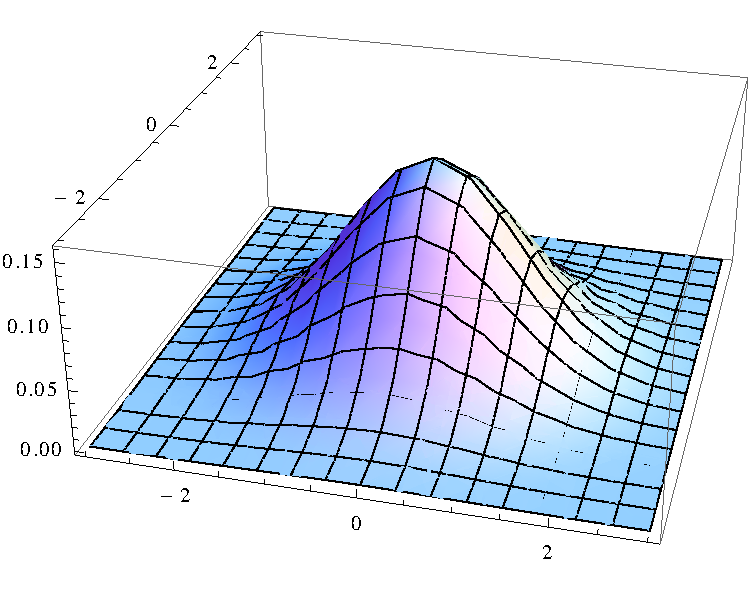
\includegraphics[scale=0.40]{multivariate.pdf}
\end{figure}
\\
This figure has mean zero for both $X_1$ and and $X_2$, and
which are independent, implying $\sigma = I_2$, the identity matrix.
It's easy to see that any vertical cuts parallel to $xz$ or $yz$ planes
will yield a traditional normal random variable. This of course
generalizes to higher dimensions, although we can't display it so nicely.
\\
\\
This generalization will give us the
\emph{Multivariate Normal (MVN) Distribution}.
This turns out to be an extremely useful distribution. Let's highlight
a few applications here:
\begin{enumerate}
  \item The MVN distribution has applications in Bayesian multivariate
    regressions (i.e. Bayesian regressions with more than one
    ``independent,'' ``predictor,'' or ``$X$'' variable).  In such
    applications, we hope to find the posterior distribution of the
    $\beta$ regression vector, and it's common to assume a MVN prior on
    $\beta$ that results in an MVN posterior for $p(\beta|y)$.

  \item Next, we often use the MVN distribution to describe
    \emph{recurrence relations}, where we try to forecast an MVN RV one
    period into the future, given current information about the RV, like
    it's current value and distribution. One example would include
    jointly forecasting height \emph{and} weight in the future given
    current height and weight.

  \item Finally, the MVN distribution forms the basis for VARs, which
    are used to forecast different economic variables one period into
    the future, expressing each future variable as a function of lags of
    itself and other economic variables.  However, VARs are too broad
    and interesting a subject to elicit only a cursory summary in this
    note.  I'll write a more extensive summary of them elsewhere.
\end{enumerate}

In this note, the multivariate distribution will apply to a
$d$-dimensional random vector
\[ X = \begin{pmatrix} X^{(1)} & X^{(2)} & \ldots & X^{(d)} \end{pmatrix}^T,
    \qquad X  \sim N_d(\mu, \Sigma) \]
where $\mu$ is the $n$-dimensional \emph{mean vector},
\[ \mu = \begin{pmatrix} EX^{(1)} & EX^{(2)} & \ldots & EX^{(d)} \end{pmatrix}^T,
      \]
and where $\Sigma$ is the $d\times d$ \emph{covariance matrix}, which
is defined and has in its $i,j$ entry
\[ \sigma^2 = E\left[ (X - \mu) (X-\mu)^T\right] \in
   \mathbb{R}^{N\times N} \]
\[ \Sigma_{ij} = Cov(X^{(i)}, X^{(j)}), \qquad i,j = 1, \ldots, d\]
Superscripts with parentheses, like ``$X^{(i)}$,'' will denote
$i$th element of the MVN RV ``$X$,'' while ``$X_t$'' will denote
an MVN RV at time $t$.


\begin{defn}(Multivariate Normal)
A random vector $X$ has a \emph{multivariate normal}
distribution if every linear combination of its components,
\[ Y = a_1 X^{(1)} + \ldots + a_d X^{(d)} \]
\[ \Leftrightarrow Y = {a} X, \qquad
    {a} \in \mathbb{R}^{d} \]
is \emph{univariate normally
distributed}, with a corresponding mean and variance. This gives a
joint density function of
\begin{equation}
    \label{pdf2}
    f_{X}({x}) = \frac{1}{(2\pi)^{d/2}\lvert \Sigma \rvert^{1/2}}
	\; e^{ -\frac{1}{2} ({x} - \mu)^T \;
	\Sigma^{-1} ({x} - \mu) }, \qquad \lvert\Sigma\rvert =
      \det\Sigma \qquad x \in \mathbb{R}^d
\end{equation}
Note, we impose the requirement that $\Sigma$ is symmetric and positive
definite.  Symmetric because the correlation of $X$ and $Y$ equals the
correlation of $Y$ and $X$.
\end{defn}
{\sl Terminology}: I'll often us MVN to refer to the case where $X$ is
a vector with $d\geq2$; however, it should be clear that the univariate
normal distribution is just a special case where $d=1$. Therefore,
when speaking about an RV that could be either MVN or univariate normal
\emph{or} properties that apply equally well to either
type of RV, I'll often use the term \emph{Gaussian}
both for convenience and out of reverence to long-dead German-speaking
mathematicians. Stimmt?


It's fairly common to consider linear transformations and functions
of a multivariate normally distributed random variable.  For instance,
we might have an economic or statistical model with a recurrence
relation to describe the dynamics of some process:
\[ X_{t+1} = A X_{t} + {V}_{t} \]
where ${V}_t$ is some innovation or random noise vector.
Therefore, it would be useful to be able to derive the distributions
of \emph{functions} or \emph{linear transformation} of multivariate
normal random variables.

So let's find the probability distribution of a linear transforamtion
of an MVN RV. Begin by assuming
\begin{align*}
    X &= A{Y}, \qquad {Y} \sim
	\text{MVN}(\mu, \Sigma) \\
    \Rightarrow \quad f(y) &= k \; \exp\left\{-\frac{1}{2} (y - \mu)^T
	\; \Sigma^{-1} (y-\mu)\right\}
\end{align*}
where $k$ is a constant.\footnote{The constant will come from the
definition of the distribution given above in Equation \ref{pdf}, but
it's boring algebra not that interesting, so I'll suppress the details.}
Assuming that $A$ is invertible, we substitute in, using Equation
, to get the distribution of $X$:
\begin{align}
    \label{midway}
    \Rightarrow \quad f_X(A^{-1}x) &= k' \exp\left\{-\frac{1}{2} (A^{-1}x - \mu)^T
	\Sigma^{-1} (A^{-1}x-\mu)\right\}
\end{align}
Next, since the expectation is a linear operator, we can use the fact
that
\begin{align*}
    EX &= E[A{Y}] = A E{Y} = A \mu \\
    \Rightarrow \quad \mu_* &= A \mu \\
    \Leftrightarrow \quad \mu &= A^{-1} \mu_*
\end{align*}
where $\mu'$ is the mean vector of $X$.  With that, we
can substitute back into Equation \ref{midway} and simplify even
further, using convenient matrix manipulations like the distributivity
property, associativity, etc.:
\begin{align*}
    f_X(A^{-1}x) &= k' \exp\left\{-\frac{1}{2} (A^{-1}x - \mu)^T \;
	\Sigma^{-1} (A^{-1}x-\mu)\right\} \\
    &= k' \exp\left\{-\frac{1}{2} (A^{-1}x - A^{-1}\mu_*)^T \;
	\Sigma^{-1} (A^{-1}x-A^{-1}\mu_*)\right\} \\
    &= k' \exp\left\{-\frac{1}{2} [A^{-1}(x - \mu_*)]^T \;
	\Sigma^{-1} [A^{-1}(x-\mu_*)]\right\} \\
    &= k' \exp\left\{-\frac{1}{2} (x - \mu_*)^T \; [(A^{-1})^T \;
	\Sigma^{-1} A^{-1}] (x-\mu_*)\right\} \\
    &= k' \exp\left\{-\frac{1}{2} (x - \mu_*)^T \;
	\Sigma_*^{-1} \; (x-\mu_*)\right\} \\
    \Rightarrow X &\sim  \text{MVN}(\mu_*, \Sigma_*),
    \qquad \text{where $\mu_* = A\mu$ and $\Sigma_* = A\Sigma A^T $}
\end{align*}
This is huge! It means \emph{linear transformations of MVN
RV's are themselves MVN.}


If you're familiar with the standard univariate normal RV,
then you can probably guess what the standard MVN RV is:
\begin{equation}
    {Z} \sim \text{MVN}(0, \; I_d)
\end{equation}
where $I_d$ is the $d\times d$ identity matrix.  This form for
the covariance matrix also suggests that the different components
of ${Z}$ (denoted $Z_1, Z_2, \ldots, Z_d$) are independent and
Gaussian.
\\
\\
Moreover, just like we can build from a standard univariate to
a general univariate.  To do so, we'll use the results from the
last section, since building from a standard MVN
to general MVN simply involves linear transformations of the components.
Specifically, we can express the MVN RV ${X}$ as follows
\begin{equation}
    {X} = \mu + A{Z}, \qquad {X}\sim
	\text{MVN}(\mu, AA^T)
\end{equation}
{\sl Computation}: Suppose we know that we want ${X}$ to
be MVN($\mu, \; \Sigma)$, and we can only generate ${Z}$.
How do we choose $A$ such that $AA^T = \Sigma$.  Typically, we'll
have to use something like a \emph{Cholesky Factorization}
algorithm to find the correct $A$ in the form of a lower triangular
matrix. And if $\Sigma$ is symmetric, positive definite, then
$A$ is guaranteed to exist and this approach will work.
The algorithm itself can be found in the appendix.


So to summarize, MVN (or Gaussian) RV's are particularly nice to work with because
of some convenient properties:
\begin{enumerate}
    \item Suppose that ${X}$ and ${Y}$ are \emph{univariate}
	normally distributed and independent. This then implies that they are
	\emph{jointly normally distributed}. In other words,
	$\begin{pmatrix} {X} & {Y} \end{pmatrix}$ must have a multivariate
	normal distribution.
    \item Linear functions of Gaussians are Gaussian. So if $A$
	is a constant matrix and ${X}$ is MVN, then $A{X}$
	is also MVN.
    \item Uncorrelated Gaussian random variables are independent.
    \item Conditions Gaussian's are normal. So if $X_1$ and $X_2$
	are two components of a MVN RV, ${X}$, then
	$X_1 | X_2$ is normal, and vice versa.
\end{enumerate}



\subsubsection{$\Chi^2$ Distribution}

\paragraph{Density Function and Descriptive Statistics}
Suppose that $Y$ has a $\chi^2$ distribution with $\nu$ degrees
of freedom. Then the distribution is a special case of the gamma
distribution, where $\alpha = \nu/2$ and $\beta = 1/2$ with the pdf
and descriptive statistics
\begin{equation}
   f_Y(y) = \frac{1}{2^{\frac{\nu}{2}} \Gamma\left(\frac{\nu}{2}\right)}
      x^{\frac{\nu}{2} - 1} e^{-\frac{x}{2}} \qquad
\text{Mean} = \nu, \qquad \text{Variance} = 2 \nu
\end{equation}

\paragraph{Derivation of Density Function} As stated in the properties
section (below), we can generate a $\chi^2(\nu)$ random variable by
summing the square of $\nu$ independent N(0,1) random variables. This
suggests that we can use an induction argument to get the distribution.

\newpage
\paragraph{Properties}
The $\chi^2$ distribution has several nice properties that we'll
want to discuss:
\begin{enumerate}
   \item If $Y$ is chi-squared distributed with $\nu$ degrees of
      freedom ($Y\sim \chi^2(\nu)$), then we can generate $Y$ by
	 \[ Y = \sum^\nu_{i=1} Z^2_i, \qquad
	    Z_i \sim N(0,1)\]
   \item By the way we just defined a $\chi^2$ RV, it's immediately
      clear that sums of $\chi^2$ RVs are also $\chi^2$ distributed.
	 \[ Y_i \sim \chi^2(\nu_i) \quad \Rightarrow \quad
	    \sum^n_{i=1} Y_i \sim \chi^2\left(\sum^n_{i=1} \nu_i \right)
	    \]
   \item Suppose that $Y_i \sim \text{NID}(\mu,\sigma^2)$. Then
       $\sum^n_{i=1} \frac{(Y_i-\mu)^2}{\sigma^2}  \sim \chi^2(n)$.
   \item Now let's suppose only the sample mean is available and
      see what we get
      \begin{align*}
	 \sum^n_{i=1} \frac{(Y_i-\mu)^2}{\sigma^2} &= \frac{1}{
	    \sigma^2} \sum^n_{i=1} (Y_i - \bar{Y}+ \bar{Y}-\mu)^2 \\
	    &= \frac{1}{\sigma^2} \sum^n_{i=1}  (Y_i - \bar{Y})^2
	    + \frac{2}{\sigma^2} \sum^n_{i=1} (Y_i-\bar{Y})(\bar{Y}-\mu)
	    + \frac{1}{\sigma^2} \sum^n_{i=1} (\bar{Y}-\mu)^2 \\
	    &= \frac{1}{\sigma^2} \sum^n_{i=1}  (Y_i - \bar{Y})^2
	    + \frac{2(\bar{Y}-\mu)}{\sigma^2} \sum^n_{i=1} (Y_i-\bar{Y})
	    + \frac{n(\bar{Y}-\mu)^2 }{\sigma^2}  \\
	 &= \sum^n_{i=1}\frac{(Y_i - \bar{Y})^2 }{\sigma^2} + 0 +
	    \left(\frac{\bar{Y}-\mu }{\sigma /\sqrt{n}}\right)^2
      \end{align*}
      Now it's clear that the left hand side is a sum of squared normal
      random variables, so it has a $\chi^2(n)$ distribution. On
      the right hand side, the third term has a $\chi^2(1)$
      distribution, as it is a squared normal random variable.
      Rearranging, we see
      \[ \sum^n_{i=1}\frac{(Y_i - \bar{Y})^2 }{\sigma^2}  \sim
	    \chi^2(n-1) \]
\end{enumerate}

\subsubsection{Beta Distribution}

One particularly useful random variable is the Beta Distribution, which
model proportions relatively well, as it only takes values between
$0$ and $1$, and which also retains the uniform distribution as a special
case.

A random variable $Y$ has a \emph{beta probability distribution} if
and only if it has density function
\begin{equation}
   \label{pdf}
   f_Y(y) = \begin{cases} \frac{y^{\alpha -1} (1-y)^{\beta-1}}{B(\alpha,
      \beta)}, & 0\leq y \leq 1 \\
	 0, & \text{otherwise}
   \end{cases} \qquad \alpha, \beta > 0
\end{equation}
where the function $B$ is defined
   \[ B(\alpha, \beta) = \int^1_0 y^{\alpha-1}(1-y)^{\beta-1} \; dy =
      \frac{\Gamma(\alpha)\Gamma(\beta)}{\Gamma(\alpha + \beta)} \]
Varying $\alpha$ and $\beta$ can lead to a vast array of different
shapes.

By a few easy manipulations, it can be shown that the beta distribution
has mean and variance
\begin{equation}
   \label{beta}
    \mu = \frac{\alpha}{\alpha+\beta}, \qquad \sigma^2 =
      \frac{\alpha\beta}{(\alpha+\beta)^2 (\alpha+\beta+1)}
\end{equation}

The Beta Function can be defined as
\[ B(\alpha, \beta) = \frac{\Gamma(\alpha) \Gamma(\beta)}{\Gamma(\alpha
   + \beta)} \]
This happens to have several integral representations, two of which
we list:
\begin{align}
   B(\alpha, \beta) &= \int^{\infty}_0 t^{\alpha-1} (1+t)^{-(\alpha+
   \beta)} \; dt \label{int1} \\
   B(\alpha, \beta) = \int^1_0 t^{x-1} (1-t)^{y-1} dt \label{int2}
\end{align}
The proof\footnote{All proofs and further information can be found
   on the Statlect.com website:
   \url{http://www.statlect.com/subon2/betfun1.htm}. }
that Equation \ref{int1} does indeed equal that of \ref{int1}
requires a bit of clever manipulation, while the Equation \ref{int2} uses
Equation \ref{int1} and makes the substitution
   \[ s = \frac{t}{1+t} = 1-\frac{1}{1+t}, \qquad \Rightarrow
      t = \frac{s}{1-s} \]


\subsubsection{General Gamma Function}

The gamma function has many special cases, but let's consider it
in its most general form, along with the mean and variance:
\begin{equation}
   f_X(x) = \frac{\beta^\alpha}{\Gamma(\alpha)} x^{\alpha-1}
      e^{-\beta x}, \qquad x > 0
\end{equation}
\[ \text{Mean} = \frac{\alpha}{\beta} \qquad \text{Variance} =
   \frac{\alpha}{\beta^2} \]
Gamma random variables also have the nice property that
\[ X_i \sim \text{Gamma}(\alpha_i, \;\beta) \quad \Rightarrow \quad
   \sum^n_{i=1} X_i \sim \text{Gamma}\left(\sum^n_{i=1} \alpha_i,\;\beta
   \right) \]

\subsubsection{Special Case: Exponential Random Variable}

This family has $\alpha=1$ with $\beta$ unrestricted. Changing the way
we denote the variables (set $\beta =\theta$), this simplifies to
   \[ f_X(x) = \theta\; e^{-\theta} \]
This is particularly useful for waiting times, as it is a memoryless
distribution. In addition, as it is technically a Gamma random
variable, sums of exponential variables will have a Gamma distribution:
\[ X_i \sim \text{Exp}(\theta) \quad \Rightarrow \quad
   \sum^n_{i=1} X_i \sim \text{Gamma}(n, \theta) \]
Another attraction is the intimate connection this distribution has
with the Poisson process.  Namely, suppose $N(t)$ is a Poisson process
with parameter $\theta$, in which case $N(t)$ is Poisson distributed
with parameter $\theta t$, then the interarrival times are
exponentially distributed with parameter $\theta$.


\subsubsection{Special Case: Chi-Squared Random Variable}

\subsubsection{Density Function and Descriptive Statistics}
Suppose that $Y$ has a $\chi^2$ distribution with $\nu$ degrees
of freedom. Then the distribution is a special case of the gamma
distribution, where $\alpha = \nu/2$ and $\beta = 1/2$ with the pdf
and descriptive statistics
\begin{equation}
   f_Y(y) = \frac{1}{2^{\frac{\nu}{2}} \Gamma\left(\frac{\nu}{2}\right)}
      x^{\frac{\nu}{2} - 1} e^{-\frac{x}{2}}
\end{equation}
   \[ \text{Mean} = \nu, \qquad \text{Variance} = 2 \nu \]

\subsubsection{Properties}

The $\chi^2$ distribution has several nice properties that we'll
want to discuss:
\begin{itemize}
   \item[-] If $Y$ is chi-squared distributed with $\nu$ degrees of
      freedom ($Y\sim \chi^2(\nu)$), then we can generate $Y$ by
	 \[ Y = \sum^\nu_{i=1} Z^2_i \]
      where $Z_i$ is a standard, normal random variable.
   \item[-] By the way we just defined a $\chi^2$ RV, it's immediately
      clear that
	 \[ Y_i \sim \chi^2(\nu_i) \quad \Rightarrow \quad
	    \sum^n_{i=1} Y_i \sim \chi^2\left(\sum^n_{i=1} \nu_i \right)
	    \]
      So sums of $\chi^2$ RVs are also $\chi^2$ distributed.
   \item[-] Suppose that $Y_i \sim \text{NID}(\mu,\sigma^2)$. Then
      \[ \sum^n_{i=1} \frac{(Y_i-\mu)^2}{\sigma^2}  \sim \chi^2(n) \]
   \item[-] Now let's consider a similar situation, but where
      only the sample mean is avalable.
      \begin{align*}
	 \sum^n_{i=1} \frac{(Y_i-\mu)^2}{\sigma^2} &= \frac{1}{
	    \sigma^2} \sum^n_{i=1} (Y_i - \bar{Y}+ \bar{Y}-\mu)^2 \\
	    &= \frac{1}{\sigma^2} \sum^n_{i=1}  (Y_i - \bar{Y})^2
	    + \frac{2}{\sigma^2} \sum^n_{i=1} (Y_i-\bar{Y})(\bar{Y}-\mu)
	    + \frac{1}{\sigma^2} \sum^n_{i=1} (\bar{Y}-\mu)^2 \\
	    &= \frac{1}{\sigma^2} \sum^n_{i=1}  (Y_i - \bar{Y})^2
	    + \frac{2(\bar{Y}-\mu)}{\sigma^2} \sum^n_{i=1} (Y_i-\bar{Y})
	    + \frac{n(\bar{Y}-\mu)^2 }{\sigma^2}  \\
	 &= \sum^n_{i=1}\frac{(Y_i - \bar{Y})^2 }{\sigma^2} +
	    \left(\frac{\bar{Y}-\mu }{\sigma /\sqrt{n}}\right)^2
      \end{align*}
      Now it's clear that the left hand side is a sum of squared normal
      random variables, so it has a $\chi^2(n)$ distribution. On
      the right hand side, the second term has a $\chi^2(1)$
      distribution, as it is a squared normal random variable. We
      can rearrange to assert that
	 \[ \sum^n_{i=1}\frac{(Y_i - \bar{Y})^2 }{\sigma^2}  \sim
	    \chi^2(n-1) \]
\end{itemize}

\clearpage
\section{Inequalities}

\begin{prop}{\emph{(Jensen's Inequality)}}
Let $g$ be a function and let $X$ be some random variable. Then
\begin{align*}
  \text{$g$ convex} &\implies \E[g(X)] \geq g\left(\E[X]\right) \\
  \text{$g$ concave} &\implies \E[g(X)] \leq g\left(\E[X]\right) \\
\end{align*}
\end{prop}
\begin{proof}
Since $g$ is a convex function, given any $x$, there is a constant $a$
such that
\begin{align*}
  g(y) \geq g(x) + a (y-x)
\end{align*}
Choose $x=\E[X]$. Then we can say that there is an $a$ such that
\begin{align*}
  g(y) &\geq g(\E[X]) + a (y-\E[X])
\end{align*}
But this must also be true for $y=X$, so
\begin{align*}
  g(X) &\geq g(\E[X]) + a (X-\E[X])
\end{align*}
Now take expectation
\begin{align*}
  \E[g(X)]
  &\geq \E[g(\E[X]) + a (X-\E[X])] \\
  &= \E[g(\E[X])] + a \E[(X-\E[X])] \\
  &= g(\E[X]) + a (\E[X]-\E[X]) \\\\
  \implies \quad
  \E[g(X)] &\geq g(\E[X])
\end{align*}
Concave proof is analogous.
\end{proof}

\begin{thm}{\emph{(Markov's Inequality)}}
\label{thm:markov}
Given random variable $X$,
\begin{equation}
    \label{markov}
    \Prb\left[
      \left\lvert X\right\rvert
      \geq \varepsilon\right]
    \leq \frac{\E\left[|X|^p\right]}{|\varepsilon|^p}
\end{equation}
\end{thm}

\begin{proof}
Write out the expectation in the numerator, where $F$ is the cdf of $X$:
\begin{align*}
  \E\left[|X|^p\right]
  &= \int^\infty_{-\infty} |X|^p \; dF \\
  &= \int^{\varepsilon}_{-\infty} |X|^p \; dF
    + \int^\infty_{\varepsilon} |X|^p \; dF
\end{align*}
Next, let's just throw out the first term in the sum above to get an
inequality. Since $|X|^p$ and the cdf are always positive, we know that
we're throwing out a positive portion, which gives us inequality
\begin{align*}
  \E\left[|X|^p\right]
  &\geq \int^\infty_{\varepsilon} |X|^p \; dF
\end{align*}
Next, notice that a lower bound for $|X|^p$ over this support will be
$|\varepsilon|^p$, so we can modify the inequality again to get
\begin{align*}
  \E\left[|X|^p\right]
  &\geq  |\varepsilon|^p \int^\infty_{\varepsilon} \; dF
  = |\varepsilon|^p \; \Prb[X\geq \varepsilon] \\
  \implies \quad
  \frac{\E\left[|X|^p\right]}{|\varepsilon|^p}
  &\geq \Prb(X\geq \varepsilon)
\end{align*}
\end{proof}

\begin{cor}{\emph{(Chebyshev's Inequality)}}
Given random variable $X$, we have
\begin{equation}
  \label{chebyshev1}
  \Prb\left[
    \left\lvert X\right\rvert
    \geq \varepsilon\right]
  \leq \frac{\E\left[X^2\right]}{\varepsilon^2}
\end{equation}
or equivalently
\begin{equation}
  \label{chebyshev2}
  \Prb\left[
    \big\lvert X-\E[X]\big\rvert
    \geq \varepsilon\right]
  \leq \frac{\Var(X)}{\varepsilon^2}
\end{equation}
\end{cor}
\begin{proof}
The proof of Statement~\ref{chebyshev1} follows by taking $p=2$ in
Markov's Inequality (Theorem~\ref{markov}).
To prove Statement~\ref{chebyshev2}, define $Z=X-\E[X]$ and use that in
Markov's inequality with $p=2$ on $Z$.
\end{proof}

\clearpage
\section{Large Sample Theory}


\subsection{Types of Convergence}

Recall the usual Analysis definition of convergence of a sequence: A
sequence $\{x_n\}$ converges to limit $x$ if for all $\varepsilon> 0$,
there exists a finite $N$ such that
\begin{align*}
  n > N \implies ||x_n - x|| < \varepsilon
\end{align*}
But this, of course, is for a sequence of numbers $\{x_n\}$ in some
metric space. There's no randomness there. So what about a sequence of
random variables---something non-deterministic?

There are a few options when talking about convergence of random
variables, but all involve resolving the randomness somehow and checking
convergence of functions, probabilities, or expectations---all of which
are possible given the usual analysis machinery.
\begin{enumerate}
  \item \emph{Almost Sure Convergence}: Check that the set of points
    $\omega\in\Omega$ where the sequence $X_n(\omega)\not\ra
    X(\omega)$ has probability zero.
  \item \emph{Convergence in Probability}: The sequence of probabilities
    that $X_n(\omega)$ is far from $X(\omega)$ over all $\omega$ goes to
    zero.
  \item \emph{Converge in $p$-Norm}: The sequence of expected distances
    $\E[|X_n-X|^p]$ goes to zero.
\end{enumerate}
In all of these cases, we've framed convergence of random variables in
terms of convergence of functions or numerical sequences. We can then
easily work with the usual analysis definitions. Now onto the formal
definitions.

\begin{defn}{(Almost Sure, Almost Everywhere, or Strong Convergence)}
Given a sequence of random variables $\{X_n\}$ and a random variable
$X$, we say that ``$X_n$ \emph{converges almost surely} to $X$'' written
\begin{align*}
  X_n\asto X
  \quad \iff \quad
  \Prb\left[\limn X_n = X\right]
  = \Prb\left[\,\omega \,\big|\,\limn X_n(\omega) = X(\omega)\right]
  = 1
\end{align*}
This checks that the number of $\omega$'s where
$\limn X_n(\omega)\neq X(\omega)$ is zero, i.e.\ that $X_n$ matches $X$
almost everywhere on $\Omega$.
Note the function can differ arbitrarily on sets that have measure zero,
or zero probability of occurring. But on those events that will occur
with some nonzero probability, $X_n$ matches $X$.  If $X_n$ and $X$ are
vectors, we need almost surely convergence element-by-element.

This notion is called ``strong convergence'' because it it computes the
probability of the limit of a sequence of random variables, rather than
the limit of a sequence of probabilities. We're effectively asking that
the random variable \emph{itself}, which is a function on sample space
$\Omega$, converges pointwise to another function on $\Omega$---the
random variable $X$---almost everywhere on $\Omega$.
\end{defn}


\begin{defn}{(Convergence in Probability)}
We say that a sequence of random variables $\{ X_n \}$ on measure space
$(\Omega,\calF,\Prb)$ \emph{converges in probability} to $X$ if
\begin{equation}
  \label{plim}
  X_n\pto X
  \quad\iff\quad
  \limn p_n(\varepsilon) :=
  \limn
  \Prb(\left\lvert X_n - X \right\rvert > \varepsilon) = 0
  \qquad \forall  \varepsilon> 0
\end{equation}
This is sometimes written as $\plim X_n = X$.
If $X_n$ and $X$ are vectors, we need convergence in probability
element-by-element.


Convergence in probability is also known as \emph{weak convergence}
because it doesn't ask the random variables (functions) $X_n$ to
converge to the random variable (function) $X$, i.e.\ that
$\limn X_n(\omega)=X(\omega)$ identically for all $\omega\in\Omega$.
Instead, we just stipulate that the realizations are very close to $X$
as $n\rightarrow\infty$.
\end{defn}

\begin{defn}{(Mean Square and $p$-norm Convergence)}
We say that a sequence of random variables $\{ X_n \}$
\emph{converges in $p$-norm} to $X$, written
\begin{align*}
  X_n \Lpto X
  \quad\iff\quad
  \limn \E\left[|X_n-X|^p\right] = 0
\end{align*}
The special case where $p=2$ is called \emph{mean square convergence} or
\emph{convergence in quadratic mean}, and is often written $X_n\msto X$.
If $X_n$ and $X$ are vectors, we need convergence in $p$-norm
element-by-element.
\end{defn}


\begin{defn}{(Convergence in Distribution or Weak Convergence)}
\label{defn:convergeInDistribution}
We say that a sequence of random variables $\{X_n\}$
\emph{converges in distribution} to random variable $X$, written
\begin{align*}
  X_n\dto X
  \quad\iff\quad
  \limn F_{X_n}(x) = F_X(x)
\end{align*}
for all values of $x$ where $F_x$ is continuous,
where $F_{X_n}$ and $F_X$ are the cdfs of $X_n$ and $X$, respectively.
If $X_n$ and $X$ are vectors, then we can characterize convergence
in distribution as either
\begin{itemize}
  \item The joint cdf of $X_n$ converges to the joint CDF of $X$.
  \item Cramer-Wold Device: $a'X_n \dto a'X$ for any non-stochastic
    vector $a$.
\end{itemize}
\end{defn}
\begin{ex}
To see why we need to restrict convergence to points of continuity on
$F_X(x)$, consider the following example:
\begin{align*}
  F_{X_n}(x) &= \one_{\left\{x\geq \frac{1}{n}\right\}}\\
  F_{X}(x) &= \one_{\left\{x\geq 0\right\}}
\end{align*} In other words, random variable $X_n$ takes on value
$\frac{1}{n}$ with probability one, while $X$ takes on value zero with
probability one.  So if we check convergence of the CDFs at $x=0$, we
have a sequence $\{F_{X_n}(0)\}_{n=1}^\infty=\{0\}_{n=1}^\infty$, which
clearly does not converge to $F_X(0)=1$.

However, it is the case that $F_{X_n}$ is well-approximated by $F_X$ at
all other points, so we'd like to be able to say $X_n\dto X$. And we
can, if we simply restrict ourselves to points where $F_X$ is
continuous.
\end{ex}

\begin{prop}
Sequence of random variables $\{X_n\} \dto X$ if and only if
\begin{align*}
  \E[g(X_n)] = \E[g(X)]
\end{align*}
\end{prop}
\begin{rmk}
This is another useful way to characterize to characterize convergence
in distribution aside from Definiton~\ref{defn:convergeInDistribution}.
It's extremely handy for a lot of results.
\end{rmk}

\begin{prop}
Given a sequence of random variables $\{X_n\}$ and random variable $X$,
the various convergence concepts are related in the following way:
\begin{enumerate}
  \item $X_n\asto X \implies X_n\pto X$. Converse not true in general.
  \item $X_n\Lpto X \implies X_n\pto X$
  \item Any one of
    \begin{align*}
      \begin{rcases}
        X_n&\asto &X \\
        X_n&\pto &X \\
        X_n&\Lpto &X
      \end{rcases}
      \implies X_n\dto X
    \end{align*}
    We see here even more explicitly that converge in distribution is
    \textsc{super weak}.
  \item Almost Surely and $p$-norm, undecidable.
  \item $X_n\pto X \implies$ There's a deterministic subsequence such
    that $X_{n_k}\asto X$ (but does not imply almost sure convergence
    for the original sequence).
\end{enumerate}
\end{prop}
\begin{proof}
We prove each in turn.
\begin{enumerate}
  \item
    %Suppose that $X_n \asto X$. Suppose also that $\varepsilon$ and
    %$\delta$ are given. Convergence in probability means that we can
    %find an $N$ such that
    %\begin{align*}
      %n>N
      %\implies
      %P(|X_n-X|>\varepsilon) < \delta
    %\end{align*}
    %Since $X_n$ converges to $X$ almost surely, for any $\omega$, there
    %is an $N_\omega$ such that
    %\begin{align*}
      %n > N_\omega
      %\implies
      %|X_n(\omega)-X(\omega)| < \varepsilon
    %\end{align*}

  \item Define random variable $Z=X_n-X$. Suppose that $\varepsilon$ is
    given. From Markov's inequality,
    \begin{align*}
      P(|Z| \geq \varepsilon) \leq \frac{\E[|Z|^p]}{|\varepsilon|^p}
      \implies
      P(|X_n-X| \geq \varepsilon) \leq \frac{\E[|X_n-X|^p]}{|\varepsilon|^p}
    \end{align*}
    As $n\ra\infty$, the righthand side of the inequality goes to zero
    since $X_n$ converges to $X$ in $p$-norm. Hence, the lefthand side
    holds.
\end{enumerate}
\end{proof}

\subsection{$O_p$ and $o_p$ Notation}

\begin{defn}(Little-$o$ Notation)
Given $\{x_n\}_{n=1}^\infty$ and $\{b_n\}_{n=1}^\infty$, we say that
\begin{align*}
  x_n = o(b_n)
  \quad \iff \quad
  \limn \frac{x_n}{b_n} = 0
\end{align*}
That is, sequence $b_n$ grows much more quickly than sequence $x_n$.
\end{defn}

\begin{defn}(Big-$O$ Notation)
Given $\{x_n\}_{n=1}^\infty$ and $\{b_n\}_{n=1}^\infty$, we say that
\begin{align*}
  x_n = O(b_n)
  \quad \iff \quad
  \exists M \; \text{s.t.} \;
  \left\lvert
  \frac{x_n}{b_n}
  \right\rvert
  < M
  \qquad \forall n
\end{align*}
That is, sequence $x_n$ grows at roughly the same rate as sequence
$b_n$, up to a scalar multiple.
\end{defn}

\begin{defn}(Little-$o_p$ Notation)
Given sequence of random variables $\{X_n\}_{n=1}^\infty$ and numerical
sequence $\{b_n\}_{n=1}^\infty$, we say that
\begin{align*}
  X_n = o_p(b_n)
  \quad \iff \quad
  \frac{X_n}{b_n} \pto 0
\end{align*}
\end{defn}

\begin{defn}(Big-$O_p$ Notation)
Given sequence of random variables $\{X_n\}_{n=1}^\infty$ and
numerical sequence $\{b_n\}_{n=1}^\infty$, we say that
\begin{align*}
  X_n = O_p(b_n)
  \quad \iff \quad
  \forall \varepsilon>0 \quad
  \exists M_\varepsilon
  \; \text{s.t.} \;
  \Prb\left(
  \left\lvert
  \frac{X_n}{b_n}
  \right\rvert
   < M\right)
  > 1- \varepsilon
  \qquad \forall n
\end{align*}
\end{defn}


\subsection{Slutsky's Theorem and the Continuous Mapping Theorem}

\begin{thm}{\emph{(Slutsky's Theorem)}}
Suppose that we have sequences of random variables $\{X_n\}$ and
$\{Y_n\}$ such that
\begin{align*}
  X_n &\dto X
  \qquad
  Y_n \pto c
\end{align*}
Then we have
\begin{enumerate}
  \item $X_n+Y_n\dto X+c$
  \item $X_n\cdot Y_n\dto Xc$
  \item $X_n/Y_n\dto X/c$ provided $c\neq 0$
\end{enumerate}
\end{thm}

\begin{cor}
Suppose that $X_n - Y_n\pto 0$ and $Y_n\dto Y$. Then $X_n \dto Y$ as
well.
\end{cor}
\begin{proof}
Define $Z_n := X_n - Y_n$. We're told that $Z_n\pto 0$. We also know
that $Y_n\dto Y$. Then by Slutsky's Theorem, we know
\begin{align*}
  Z_n + Y_n &\dto 0 + Y \\
  \Leftrightarrow\quad (X_n-Y_n) + Y_n &\dto 0 + Y \\
  \Leftrightarrow\quad X_n &\dto Y
\end{align*}
\end{proof}

\begin{thm}\emph{(Continuous Mapping Theorem)}
Let $g$ be a continuous function. Then
\begin{enumerate}
  \item $X_n\dto X \implies g(X_n) \dto g(X)$
  \item $X_n\pto X \implies g(X_n) \pto g(X)$
\end{enumerate}
\end{thm}

%Now for some final notes. Convergence in probability
%is \textbf{not} convergence in expectation. The former
%concerns a sequence of probabilities, while the latter a
%sequence of expectations. Finally, the probability limit
%$X$ must be free of all dependence upon the sample size $n$.

\subsection{Law of Large Numbers}

\begin{thm}\emph{(Weak Law of Large Numbers)}
Given a sequence $\{X_n\}$ of random variables such that
$\E[X_n]=\mu$, $\Var(X_n)=\sigma^2$, and $\Cov(X_i,X_j)=0$,
\begin{align*}
  \hat{\mu}_N \pto \mu
  \qquad\text{where} \quad
  \hat{\mu}_N := \frac{1}{N} \sumnN X_n
\end{align*}
\end{thm}
\begin{rmk}
We assume existence of the second moment here. In the Strong Law of
Large Numbers, we dispense with that assumption.
\end{rmk}
\begin{proof}
Since $\hat{\mu}_N$ is a random variable, we can use Chebyshev's
inequality. Fix $\varepsilon$. Then
\begin{align*}
  \Prb(|\hat{\mu}_N -\mu| \geq \varepsilon)
  \leq \frac{\Var(\hat{\mu}_N)}{\varepsilon^2}
\end{align*}
Note that $\Var(\hat{\mu}_N) = \frac{\sigma^2}{N}$, which implies
\begin{align*}
  \Prb(|\hat{\mu}_N -\mu| \geq \varepsilon)
  \leq \frac{\sigma^2}{N\varepsilon^2}
\end{align*}
As $N\ra\infty$, the object on the right goes to zero. Since
$\varepsilon$ was arbitrary, we have exactly what we need to say that
$\hat{\mu}_N\ra\mu$.
\end{proof}

\begin{thm}\emph{(Strong Law of Large Numbers)}
Suppose that $\{X_n\}$ is a sequence of iid random variables with mean
$\E[X_n]=\mu$.
\begin{align*}
  \hat{\mu}_N \asto \mu
  \qquad\text{where} \quad
  \hat{\mu}_N := \frac{1}{N} \sumnN X_n
\end{align*}
\end{thm}


\subsection{Central Limit Theorem}

\begin{thm}
Let $\{X_i\}_{i=1}1^n$ be a sequence of iid random variables with
$\E[X_i] = \mu$ and $\Var(X_i)=\sigma^2$. Then
\begin{align*}
  \frac{\sqrt{n}}{\sigma}
  \left(\bar{X}_n - \mu\right) \dto N(0,1)
  \quad
  \bar{X}_n := \frac{1}{n}\sumin X_i
\end{align*}
\end{thm}


\clearpage
\subsection{Delta Method}

Suppose that we have random variable $\bsy\in \mathbb{R}^m$,
with mean and variance-covariance matrix as follows:
\begin{align*}
  \bsmu &:= \mathbb{E}(\bsy) =
  \begin{pmatrix}
    \mathbb{E}(y_1)\\\mathbb{E}(y_2)\\\vdots\\\mathbb{E}(y_m)
  \end{pmatrix}
  \in \mathbb{R}^m
  \\
  \bsSigma
  &:=
  \mathbb{E}\left[ (\bsy-\bsmu) (\bsy-\bsmu)' \right]
  \in \mathbb{R}^{m\times m}
\end{align*}
Now suppose that we have an iid sample $\left\{\bsy_i\right\}_{i=1}^N$.
We can construct an estimator of the first moment vector
\begin{align*}
  \bshatmu
  &=
  \frac{1}{N}
  \sum^N_{i=1}
  \bsy_i\\
  \sqrt{N}(\bshatmu - \bsmu)
  &\dto N(0,\Sigma)
\end{align*}
where the convergence of this estimator follows from the Central Limit
Theorem.

Now consider a transformation of the first moment vector, denoted
$\bsg(\bsmu)$.  We want a sampling distribution for that guy too (mean
and standard errors), just like we had one for $\bsmu$.  The \emph{delta
method} allows us to do that.

One quick thing to note: The fact that $\bsg(\bsmu)$ is only a function
of the first moment of $\bsy$ isn't that restrictive if we're willing to
generalize our notion of $\bsy$. We can easily accommodate more
complicated moments with a minor tweak.

To see this, suppose that we have some base random variable
$\bsx\in\mathbb{R}^n$
\begin{align*}
  \bsx =
  \begin{pmatrix}
    x_1\\x_2\\\vdots\\x_n
  \end{pmatrix}
  \in \mathbb{R}^n
\end{align*}
along with sample $\{\bsx_i\}_{i=1}^N$. If we want second
moments or cross-correlations of elements in $\bsx$, simply
define a function $\bsh: \mathbb{R}^n \rightarrow
\mathbb{R}^m$ to do the transformations you want and set
\begin{align*}
  \bsy
  :=\bsh(\bsx)
  =
  \begin{pmatrix}
    h_1(\bsx)\\h_2(\bsx)\\\vdots\\h_m(\bsx)
  \end{pmatrix}
  \in\mathbb{R}^m
\end{align*}
Then, to generate the sample for $\bsy$, just take
\begin{align*}
  \{\bsy_i\}_{i=1}^N &:=
  \left\{\bsh\left(\bsx_i\right)\right\}_{i=1}^N
\end{align*}
From there, proceed exactly as before. In this way, we can always use
the ``first moment representation'' above, leaving open the possibility
that $\bsy$ is actually a transformation or function of some
base random variable.


\begin{thm}\emph{(Delta Method)}
Let $\bshatmu_N$ denote the mean of iid sample
$\{\bsy_i\}^N_{i=1}$ for random variable $\bsy$.
The central limit theorem tells us that as $N\rightarrow\infty$,
\begin{align*}
  \sqrt{N}\left(
  \bshatmu_N
  -\bsmu
  \right)
  \xrightarrow{d} N(0, \bsSigma)
\end{align*}
For continuously differentiable transformation $\bsg:\R^m\rightarrow
\R^p$, the \emph{delta method} states that
\begin{align*}
  \sqrt{N}\left(
  \bsg(\bshatmu_N)
  -
  \bsg(\bsmu)
  \right)
  &\xrightarrow{d} N\left(
    0, \bsG \bsSigma \bsGp
  \right)\\\\
  \text{where}\quad
  \bsJ(\bsu)
  &:=\frac{\partial}{\partial \bsup}
  \left[\bsg(\bsu)\right]\\
  \text{and} \quad
  \bsG &:= \bsJ(\bsmu)
\end{align*}
In words, suggestively-named $\bsJ$ is the Jacobian of $\bsg$, while
$\bsG$ is shorthand for the Jacobian evaluated at the true value
$\bsmu$.
\end{thm}
\begin{proof}
Start by using the mean value theorem about the true value $\bsmu$:
\begin{align*}
  \bsg(\bshatmu_N)
  &=
  \bsg(\bsmu)
  + \bsJ(\tilde{\bsmu}) \left( \bshatmu_N - \bsmu \right)\\
  \Leftrightarrow\quad
  \bsg(\bshatmu_N) - \bsg(\bsmu)
  &=
  \bsJ(\tilde{\bsmu}) \left( \bshatmu_N - \bsmu \right)
\end{align*}
where $\tilde{\bsmu}$ is in between $\bsmu$ and $\bshatmu_N$.
But we know that
\begin{align*}
  \bshatmu_N \pto \bsmu
  \quad\implies\quad
  \tilde{\bsmu} \pto \bsmu
\end{align*}
Then, since $\bsg$ is continuously differentiable, the Jacobian is
continuous, so by the Continuous Mapping Theorem
\begin{align*}
  \tilde{\bsmu} \pto \bsmu
  \quad\implies\quad
  \bsJ(\tilde{\bsmu})
  \pto \bsJ(\bsmu) = \bsG
\end{align*}
From there, we can use this in Slutsky's Theorem:
\begin{align*}
  \begin{rcases}
  \sqrt{N}\left(\bshatmu_N-\bsmu\right) &\dto N(0,\bsSigma) \\
  \bsJ(\tilde{\bsmu}) &\pto \bsG
  \end{rcases}
  \quad\implies\quad
  \bsG \sqrt{N} (\bshatmu-\bsmu) \dto
  \bsG \bsX
  \sim N(0,\bsG \bsSigma \bsG')
\end{align*}
where I used $\bsX\sim N(0,\bsSigma)$ to stand in for the limiting
distribution of $\sqrt{N}(\bshatmu_N-\bsmu)$.
But notice by the mean-value theorem expansion we did above, we have
now enough to conclude that
\begin{align*}
  \sqrt{N} \bsG (\bshatmu-\bsmu)
  = \sqrt{N}(\bsg(\bshatmu_N)-\bsg(\bshatmu))
  \dto N(0,\bsG \bsSigma \bsG')
\end{align*}
which is exactly what we wanted to prove.
\end{proof}

\section{Estimators}


Most of statistics is about optimally estimating parameters using
observed data. In this section, we develop language to talk about that.
The key concepts are \emph{estimators} of parameters, \emph{loss} which
defines a quantitative penalty for poor estimates, and \emph{risk} which
characterizes expected loss---an average of the loss using some suitable
weighting function. You can write down many loss functions. We will also
see a few definitions of risk which reflect different weighting
functions.

\begin{defn}(Estimator)
An \emph{estimator} $\hat{\theta}$ of parameter $\theta$ is a
function $\hat{\theta}: \RN \ra \R$.
It maps $N$ random variables representing sample points into a guess for
$\theta$. Since the sample is random, $\hat{\theta}(Y_1,\ldots,Y_N)$ is
itself a random variable.
\end{defn}

\begin{defn}(Estimate)
Given a realizations $y_1,\ldots,y_N$, we can form an
\emph{estimate}---a computed value that is actually a number---by
plugging in the sample $\{y_n\}^N_{n=1}$ into $\hat{\theta}$.
\end{defn}

\begin{defn}(Loss Function)
The \emph{loss function} $L(\hat{\theta},\theta)$ is a function that
maps the true parameter value $\theta$ and an estimator $\hat{\theta}$
into negative utility. It returns the ``loss''---a number---quantifying
how bad it was to use $\hat{\theta}$ when the true value was $\theta$.
We can think of it as a penalty function in the search for good
estimators.
\end{defn}

\begin{defn}{(Classical or Frequentist Risk Function)}
Given loss function $L(\hat{\theta},\theta)$, the \emph{classical} or
\emph{frequentist risk function} is the expected value of the loss:
\begin{align*}
  R(\hat{\theta},\theta) = \E_{Y|\theta}[L(\hat{\theta},\theta)]
\end{align*}
Conditional on a value of $\theta$, this expectation will average out
over the values $\hat{\theta}$ takes on. (Recall, is a random variable
as a function of $Y_1,\ldots,Y_N$.) The ``Classical'' and
``Frequentist'' qualifiers follow from the fact that
$R(\hat{\theta},\theta)$ does not integrate over different values that
$\theta$ can take on, since frequentists want to treat $\theta$ as a
fixed constant, not a random variable.
\end{defn}
\begin{rmk}
In general, $\theta$ will be unknown. So the whole game for frequentists
is about finding estimators $\hat{\theta}$ that are robust to many
different values of $\theta$. That's why we tend to like estimators with
small bias and small variance. Bayesians take a different approach,
integrating over the different values of $\theta$, which we'll see in
the definition of \emph{Bayes risk} below.
\end{rmk}

\begin{ex}(Quadratic Loss and Mean Squared Error)
Often, a good loss function is the \emph{quadratic loss} function
\begin{align*}
  L(\hat{\theta},\theta) = (\hat{\theta}-\theta)^2
\end{align*}
which penalizes more steeply the further away you are from the true
value. It has associated \emph{mean squared error} risk:
\begin{align*}
  R(\hat{\theta},\theta) = \E_{Y|\theta}[(\hat{\theta}-\theta)^2]
\end{align*}
\end{ex}

\begin{defn}(Bayes Risk)
\label{defn:bayesrisk}
Given a prior distribution $w(\theta)$ for parameter $\theta$, the
\emph{Bayes risk} denoted $r(\hat{\theta})$ averages the classical or
frequentist risk over the values of $\theta$, weighted by $w(\theta)$:
\begin{align*}
  r(\hat{\theta})
  = \int R(\hat{\theta},\theta) w(\theta) \; d\theta
\end{align*}
Note that we can express that a few different ways in terms of
expectation operators, all of which offer different type of intuition:
\begin{align*}
  r(\hat{\theta})
  = \int R(\hat{\theta},\theta) w(\theta) \; d\theta
  &= \E_\theta[ R(\hat{\theta},\theta)] \\
  &= \E_\theta\left[
      \E_{Y|\theta}\left[
      L(\hat{\theta},\theta)
      \right]
    \right] \\
  &= \E_{\theta,Y}\left[ L(\hat{\theta},\theta) \right]
\end{align*}
In words, frequentist risk $R(\hat{\theta},\theta)$ gives expected loss
conditional on a value of $\theta$, denoted
$\E_{Y|\theta}[L(\hat{\theta},\theta)]$. If you take the expectation of
that, by the law of iterated expectations, you get
$\E_{\theta,Y}[L(\hat{\theta},\theta)]$, which is the expected loss
\emph{jointly} averaging out over both data $Y$ uncertainty \emph{and}
parameter $\theta$ uncertainty.
\end{defn}
\begin{rmk}
In general, different priors or $w(\theta)$ functions will give
different estimates of Bayes risk. Choose wisely.
\end{rmk}

\begin{defn}{(Posterior Risk or Posterior Expected Loss)}
This is the expected loss conditional on $Y=y$:
\begin{align*}
  \E_{\theta|Y}[L(\hat{\theta},\theta)|Y=y]
  =
  \int L(\hat{\theta},\theta) f_{\theta|Y}(\theta|y) \; d\theta
\end{align*}
So you have a posterior $f_{\theta|y}(\theta|y)$ that characterizes the
distribution of $\theta$ after observing data $y$. The posterior risk is
an average of the loss, but using the posterior as the appropriate
weighting function. As a result, you weight the loss more heavily in
areas where the $f_{\theta|y}(\theta|y)$ is largest.
\end{defn}

\begin{ex}
To be more concrete, suppose the data $y$ suggests that $\theta$ is most
likely positive.  Then if your estimator has huge loss in negative
territory (i.e. $\hat{\theta}$ is far from $\theta$ when $\theta$ is
negative), whatever. You don't care. Discount that loss because $\theta$
probably isn't over there. We shouldn't penalize $\hat{\theta}$ if it's
does a shitty job estimating $\theta$ in regions where $\theta$ is
really unlikely to be.
\end{ex}

\begin{prop}
\label{prop:bayesrisk}
Definition~\ref{defn:bayesrisk} defines the Bayes risk as the average of
classical or frequentist risk over all values of $\theta$ weighted by
the prior. We can equivalently characterize Bayes risk as the posterior
risk averaged over all values of $Y$. In other words
\begin{align*}
  r(\hat{\theta})
  &= \E_{\theta,Y}[L(\hat{\theta},\theta)]
  =
  \begin{cases}
    \E_\theta\left[\E_{Y|\theta}[L(\hat{\theta},\theta)]\right]
    &\text{Ave.\ over classical/frequentist risk} \\
    \E_Y\left[\E_{\theta|Y}[L(\hat{\theta},\theta)]\right]
    &\text{Ave.\ over posterior risk} \\
  \end{cases}
\end{align*}
\end{prop}
%\begin{proof}
%Write out the definition or $r(\hat{\theta})$
%\begin{align*}
  %r(\hat{\theta})
  %&= \E_\theta[R(\hat{\theta},\theta)] \\
  %&= \int R(\hat{\theta},\theta)  w(\theta) \; d\theta
%\end{align*}
%\end{proof}

\begin{defn}(Bayes Estimator)
\label{defn:bayesest}
Given a loss function $L(\hat{\theta},\theta)$, the
\emph{Bayes estimator} is the estimator that minimizes posterior risk
for each $y$:
\begin{align*}
  \hat{\theta}_{\text{Bayes}}
  = \argmin_{\hat{\theta}} \; \E_{\theta|Y}[L(\hat{\theta},\theta)|Y=y]
\end{align*}
\end{defn}

\begin{prop}
The Bayes Estimator minimizes Bayes risk.
\end{prop}
\begin{proof}
Definition~\ref{defn:bayesest} defines the Bayes estimator as the
estimator that minimizes posterior risk for each $y$.
Proposition~\ref{prop:bayesrisk} defines Bayes risk as the average of
the posterior risk over all $y$. Clearly, the Bayes estimator must
minimize Bayes risk.
\end{proof}


\begin{ex}
Given quadratic loss $L(\hat{\theta},\theta) = (\hat{\theta}-\theta)^2$,
the Bayes estimator is the posterior mean:
\begin{align*}
  \hat{\theta}_{\text{Bayes}}
  &= \E_{\theta|Y}[\theta|Y=y]
\end{align*}
\end{ex}

\begin{defn}(Unbiased)
An estimator is \emph{unbiased} if
\begin{align*}
  \E\left[\,\hat{\theta}\,\right] =
  \underbrace{\int \cdots \int}_{n\; times} 
      \hat{\theta}(y_1,\ldots,y_n) \;
      f_{Y_1,\ldots,Y_n}(y_1,\ldots,y_n) \; dy_1 \ldots dy_n = \theta
\end{align*}
\end{defn}

\begin{rmk}(Bias-Variance Tradeoff)
Given estimator $\hat{\theta}$ of parameter $\theta$,
\end{rmk}

\subsection{Consistency}

\begin{defn}(Consistency)
A sequence of estimators $\{ \hat{\theta}_n \}$
where $n=1,2,\ldots$ is \emph{consistent} for parameter $\theta$ if
$\hat{\theta}_n$ converges \emph{In Probability} to $\theta$.
\end{defn}

\begin{defn}(Strongly Consistent)
If convergence of $\hat{\theta}_n$ to $\theta$ holds with probability 1.
\end{defn}


\clearpage
\section{Generalized Method of Moments (GMM)}

GMM is often done in the context of time series models, and so I will
use $T$ to denote sample size rather than $N$.

\subsection{Notation}

Suppose that we have vector random variable $\bsy_t$ with
population mean $\mathbb{E}(\bsy_t)$. Given a sample
$\{\bsy_t\}^T_{t=1}$, we can form an estimator of the mean
\begin{align*}
  \mathbb{E}_T(\bsy_t)
  := \frac{1}{T} \sum^T_{t=1} \bsy_t
\end{align*}
Oten, however, we have a model and want to estimate a vector of
parameters, $\bsb$. When this is the goal, we define a function
that suppresses some of the notation above and makes the focus on
parameters more explicit:
\begin{align*}
  \bsg(\bsb)
  &:= \mathbb{E}[\boldsymbol{f}(\bsy_t,\bsb)]\\
  \bsg_T(\bsb)
  &:= \mathbb{E}_T[\boldsymbol{f}(\bsy_t,\bsb)]
  = \frac{1}{T}\sum^T_{t=1}
      \boldsymbol{f}(\bsy_t,\bsb)
\end{align*}
where $\boldsymbol{f}$ is some function that mixes data and parameters
according to model-implied structure. We'll see more clearly how this is
used below.

But in general, note the convention: For a population concept like
$\mathbb{E}(\cdot)$ or $\bsg(\cdot)$, we form the sample
estimators (given $T$ observations) of $\mathbb{E}_T(\cdot)$ and
$\bsg_T(\cdot)$.

This convention might seem a little odd at first since
$\mathbb{E}_T(\cdot)$ is often used to denote the expectation
conditional on time $T$ information. But that's not going to be a
problem here, since GMM will deal pretty much exclusively with
\emph{unconditional} moments (or at least unconditional with respect to
time).\footnote{%
To take a quick example, consider the simple de-meaned, stationary AR(1)
model
\begin{align*}
  y_t = \rho y_{t-1} + \varepsilon_t
  \qquad \varepsilon_t \sim N(0,\sigma^2)
\end{align*}
You might reasonably care about \emph{either} the unconditional or (on
time $t-1$ information) mean and variance of $y_t$.
\begin{alignat*}{3}
  \mathbb{E}(y_t) &= 0 &\mathbb{E}_t(y_{t}) &= \rho y_{t-1}\\
  \text{Var}(y_t) &= \frac{\sigma^2}{1-\rho^2}
  \qquad
  &\text{Var}_t(y_t) &= \sigma^2
\end{alignat*}
In GMM, we'll be talking about the unconditional estimates on the left.
}
Plus, the convention has the added benefit of connecting estimators to
their sample estimates in about the most explicit way possible (i.e.\
just add ${}_T$ to go from estimator to estimate).


\subsection{Distribution of Sample Mean}
\label{sec:mean}

This is a rather straightfoward exercise, but it allows us to derive a
few important concepts in GMM notation. So let's go ahead.

Given a sample $\{\bsy_t\}^T_{t=1}$ of stationary (typically
autocorrelated) random variable $\bsy_t$, we defined an
estimator of the sample mean, $\mathbb{E}_T(\bsy_t)$. Now
let's characterize that estimator's distribution, since it too is a
random variable.

First, the mean:
\begin{align*}
  \mathbb{E}\left(\mathbb{E}_T(\bsy_t)\right)
  &= \mathbb{E}\left(\frac{1}{T}\sum^T_{t=1} \bsy_t\right)
  = \frac{1}{T}\sum^T_{t=1} \mathbb{E}\left(\bsy_t\right)
  = \frac{1}{T} \times T \; \mathbb{E}\left(\bsy_t\right)\\
  &= \mathbb{E}\left(\bsy_t\right)
\end{align*}
So $\mathbb{E}_T(\bsy_t)$ is an unbiased estimator of the
unconditional mean of $\bsy_t$.

Now we get the variance of the estimator, accounting for the fact that
the sample $\{\bsy_t\}_{t=1}^T$ is not necessarily iid (though
assumed stationary):
\begin{align}
  \text{Var}(\mathbb{E}_T(\bsy_t))
  &=
  \text{Var}\left(
  \frac{1}{T}\sum^T_{t=1} \bsy_t
  \right)
  =
  \frac{1}{T^2}\text{Var}\left(
  \sum^T_{t=1} \bsy_t
  \right)\notag\\
  &=
  \frac{1}{T^2}
  \sum^T_{j=-T} (T-|j|)\text{Cov}\left(
    \bsy_t, \bsy_{t-j}
  \right) \notag\\
  &=
  \frac{1}{T^2}
  \left[
    \sum^T_{t=1} \text{Var}(\boldsymbol{y_t})
    +
    2\sum^T_{j=1} (T-|j|)\text{Cov}(\bsy_t,\bsy_{t-j})
  \right]\notag\\
  \Rightarrow\quad
  \text{Var}(\mathbb{E}_T(\bsy_t))
  &=
  \frac{1}{T}
  \left[
    \text{Var}(\boldsymbol{y_t})
    +
    2\sum^T_{j=1} \frac{T-|j|}{T}
    \text{Cov}(\bsy_t,\bsy_{t-j})
  \right]
  \label{eq:estvar}
\end{align}
A few things to note about this last result:
\begin{enumerate}
  \item In the case of iid observations,
    $\text{Cov}(\bsy_t,\bsy_{t-j})$ will be zero for
    all $j\neq 0$, in which case we get the classic ``$\sqrt{T}$
    result'' for the standard deviation:
    \begin{align*}
      \text{Var}(\mathbb{E}_T(\bsy_t))
      &=
      \frac{\text{Var}(\boldsymbol{y_t})}{T}\\
      \Rightarrow\quad
      \sigma(\mathbb{E}_T(\bsy_t))
      &=
      \frac{\sigma(\boldsymbol{y_t})}{\sqrt{T}}
    \end{align*}
    In words, ``The average of any sample always gives a unbiased
    estimate of the mean. And when the data is uncorrelated, the
    precision of that estimate increases at a rate of $\sqrt{T}$.''

  \item When the observations are \emph{not} iid (when there is serial
    correlation in the sample), Equation~\ref{eq:estvar} says that you
    don't really have $T$ observations. The serial correlation decreases
    the number of \emph{effective} observations you have. So crank up
    the variance of your estimate, depending upon how strong that serial
    correlation is.

  \item
    You can see from Equation~\ref{eq:estvar} that when $T$ get's large,
    $\frac{T-|j|}{T}$ approaches unity, which gives
    \begin{align*}
      \lim_{T\rightarrow\infty}
      \text{Var}(\mathbb{E}_T(\bsy_t))
      &=
      \frac{1}{T}
      \left[
        \text{Var}(\boldsymbol{y_t})
        +
        2\sum^\infty_{j=1}
        \text{Cov}(\bsy_t,\bsy_{t-j})
      \right]
      =
      \frac{\bsS}{T}
    \end{align*}
    where $\bsS$ is the spectral density of $\bsy_t$
    at frequency at zero.
\end{enumerate}
From there, we can use the Central Limit Theorem to state the following
result.

\begin{thm}
Given a sample $\{\bsy_t\}_{t=1}^T$ for random variable
$\bsy_t$
\begin{align*}
  \sqrt{T}\left(
    \mathbb{E}_T(\bsy_t) -\mathbb{E}(\bsy_t)
  \right)
  \xrightarrow{d} N(0,\bsS)
\end{align*}
where $\bsS$ is the spectral density at frequency zero defined
\begin{align*}
  \bsS :=
  \sum^\infty_{j=-\infty}
    \text{\normalfont Cov}(\bsy_t, \bsy_{t-j})
  =
  \text{\normalfont Var}(\bsy_t)
  + 2 \sum^\infty_{j=1}
  \text{\normalfont Cov}(\bsy_t,\bsy_{t-j})
\end{align*}
This holds regardless of whether or not the data are iid or serially
correlated (since you're using the correct covariance matrix,
$\bsS$).
\end{thm}

\clearpage
\subsection{Casting the Model in GMM Form}

The first step is to write your model in standard GMM form:
\begin{align}
  0 &= \bsg(\bsb)\label{eq:stdform}\\
  \Leftrightarrow\qquad
  0 &= \mathbb{E}[\boldsymbol{f}(\bsy_t,\bsb)]
  \notag
\end{align}
where $\bsb\in\mathbb{R}^p$,
$\bsy_t\in\mathbb{R}^n$, and $\boldsymbol{f},
\bsg\in\mathbb{R}^m$.  Equation~\ref{eq:stdform} states the
\emph{moment conditions} of the model, since it encapsulates
restrictions the model imposes on the moments.
\\
\\
Examples
\begin{enumerate}
  \item An asset pricing model of asset ruturns for $N$ assets can be
    expressed
    \begin{align*}
      1 &= \mathbb{E}(m_{t+1}(b) \boldsymbol{R}_{t+1}) \\
      \Leftrightarrow \qquad
      0 &= \mathbb{E}(m_{t+1}(b) \boldsymbol{R}_{t+1}-1)\\
      \boldsymbol{R}_{t+1} &=
      \begin{pmatrix}
        R^1_{t+1}
        &\cdots&
        R^N_{t+1}
      \end{pmatrix}'
    \end{align*}
    where the discount factor $m_{t+1}(b)$ is a scalar that depends on
    data and model parameters.
  \item Let $\boldsymbol{f}(\bsy_t,\bsb)$ represent
    forecast or regression errors at time $t$ for a vector of different
    data series that we're trying to predict or describe with the model.
    Then Equation~\ref{eq:stdform} expresses the natural idea ``Set
    errors to zero.''
  \item Take a typical regression equation:
    \begin{align*}
    \end{align*}
\end{enumerate}
So it's usually very easy to write any model (linear or nonlinear) in
standard form. Your model's structure is going to consist of a bunch of
equations that place restrictions on data and parameters.  Simply figure
out what combination of data and parameters should be zero in
expectation, and the shift terms in those equations around as necessary
until you work your model's restrictions/implications into the standard
representation of Equation~\ref{eq:stdform}.

\clearpage
\subsection{Estimating the Model}

Suppose that your model is the correct model of the world. Then by
assumption, if we can find the \emph{true} parameter vector
$\bsb_0\in \mathbb{R}^p$, it must be the case that
\begin{align}
  \bsg(\bsb_0) = 0
  \label{eq:gmmtrue}
\end{align}
This suggests how to find an estimate $\bshatb$ of true
parameter vector $\bsb_0$: just find the vector that sets the
the function $\bsg(\bsb)$ to zero---i.e.\ solve the
system.  But in practice, we need to overcome two very obvious issues
with that recommendation.

First, we don't have access to the population moment conditions
$\bsg(\bsb)$. Remember that the function
$\bsg$ depends upon random variable $\bsy_t$ under
the hood, and we work with samples like $\{\bsy_t\}_{t=1}^T$
in real life.  But we have an easy fix for that: just set the sample
equivalent $\bsg_T(\bsb)=0$ instead. Done, this
problem is solved.  \emph{However}, that leads us right to our next
issue.

We won't be able to simply set $\bsg_T(\bsb)=0$
since the model The model probably isn't \emph{actually} the true model
of the world. And in general, we're not going to be able set all $m$
elements of vector $\bsg_T(\bsb)$ to zero with a
misspecified model when $p<m$ (when the number of free parameters $p$ is
less than the number of moment conditions $m$).  Now of course, we want
$p<m$ because models should be parsimonious with less degress of freedom
than data points, but the consequence is that you can't cleanly solve
the system to set $\bsg_T(\bsb)=0$.

So how exactly do you estimate the $p$ parameters given these issues,
sample $\{\bsy_t\}_{t=1}^T$, and corresponding vector-valued
function $\bsg_T(\bsb)\in \mathbb{R}^m$? There are
two approaches:
\begin{enumerate}
  \item Choose a matrix $\boldsymbol{a}_T\in\mathbb{R}^{p\times m}$ and
    set only $p$ linear combinations of the
    moments to zero, i.e.\ solve the system of $p$ equations for the
    $\bshatb$ that satisfies
    \begin{align}
      \boldsymbol{a}_T
      \;
      \bsg_T(\bshatb) = 0
      \label{eq:bhatdef}
    \end{align}
    Most of the time, $\boldsymbol{a}_T$ will be a matrix of ones and
    zeros to pick out the moments in $\bsg_T(b)$ (or form
    linear combination of moments) we want to force to zero. But it
    really can be as complicated as you want or depend upon sample size
    (hence the ${}_T$ subscript). We'll see an example just below.

    The main idea: $p<m$ means we can't set \emph{all} of the $m$
    moments to zero, so focus on $p$ important ones.\footnote{Of course,
      this might all be pointless if $r > g$ and patrimonial capitalism
    kills us all. ``Piketty!!! [Shakes fist at sky]''}

  \item If we don't want to take a stance on the important moments, form
    a weighting matrix $\boldsymbol{W}\in \mathbb{R}^{m\times m}$ and
    choose the parameter vector that gets the squared (weighted)
    elements of $\bsg_T(\bsb)$ as close to zero as
    possible:
    \begin{align}
      \bshatb = \arg\min_{\bsb}\;
      \bsg_T(\bsb)' \boldsymbol{W}
      \bsg_T(\bsb)
      \label{eq:bhatmin}
    \end{align}
    We're minimizing a weighted sum of squared ``errors'' (i.e.\
    differences of $\bsg_T(b)$ from its target of zero), which
    is both conceptually and computationally straightfoward.

    And, just to tie things together, this is actually equivalent to
    Approach 1, if you set
    \begin{align}
      \boldsymbol{a}_T =
      \frac{\partial \bsg'_T}{\partial \bsb}
      \boldsymbol{W}
      =
      \bsd'
      \boldsymbol{W}
      \label{eq:equivrep}
    \end{align}
    where $\bsd
    :=\frac{\partial \bsg'_T}{\partial \bsb}
    \in \mathbb{R}^{p\times m}$.
    This follows from the first order conditions to the minimization
    defined by Equation~\ref{eq:bhatmin}:
    \begin{align*}
      0
      = \frac{\partial \bsg'_T}{\partial \bsb}
      \boldsymbol{W} \bsg_T(\bsb)
      = \bsd'
      \boldsymbol{W} \bsg_T(\bsb)
    \end{align*}
    We'll talk about choices of the weighting matrix
    $\boldsymbol{W}$ later on. For now though, you might reasonably just
    choose $\boldsymbol{W}=\boldsymbol{I}$, treating all moments
    equally.
\end{enumerate}

\subsection{Standard Errors}

Next, suppose we have a sample $\{\bsy_t\}^T_{t=1}$. To get
standard errors for the various objects we will estimate, we proceed in
a sequence of steps
\begin{enumerate}
  \item Define $\bsS$, the spectral density matrix of
    population moment vector
    $\bsg(
    \bsb)=\mathbb{E}[\boldsymbol{f}(\bsy,
    \bsb)]$ for fixed $\bsb$.

    Given fixed $\bsb$, the vector
    $\bsg(\bsb)
    =\mathbb{E}[\boldsymbol{f}(\bsy_t,\bsb)]$
    is simply the mean of object
    $\boldsymbol{f}(\bsy_t,\bsb)$.
    We recall the definition from Section~\ref{sec:mean} for
    the spectral density at frequency zero:
    \begin{align*}
      \bsS = \sum^\infty_{j={-\infty}}
        \text{Cov}(\boldsymbol{f}(\bsy_t,\bsb),
          \boldsymbol{f}(\bsy_t,\bsb))
        =
        \mathbb{E}\left[
        \boldsymbol{f}(\bsy_t,\bsb)
        \boldsymbol{f}(\bsy_t,\bsb)'
        \right]
    \end{align*}
    Nothing deep there, just applying our definition from earlier. Of
    course, eventually, we'll have to talk about estimating this beast
    given a sample (since we usually won't know $\bsS$), but
    for now, let's just take it as given and work through the math for
    everything else. We'll return to it later.

  \item Use $\bsS$ to derive the standard error of sample mean
    $\boldsymbol{a}_T\bsg_T(\bsb)$ for fixed
    $\bsb$.\footnote{We compute standard errors for
      $\boldsymbol{a}_T\bsg_T(\bsb)$, not just
      $\bsg_T(\bsb)$ because we impose that the
      former equals zero, but we don't know anything about the latter.
      And we will need to use the equality
      $\boldsymbol{a}_T\bsg_T(\bsb)=0$,
      Taylor-expand the lefthand side, shuffle things around, and get
      results in the next step.}

    Just like in Section~\ref{sec:mean}, we have a sample estimate
    $\bsg_T(\bsb)$ for a population mean vector
    $\bsg(\bsb)$. We also have $\bsS$, the
    spectral density at frequency zero. Put this together to get
    \begin{align*}
      \sqrt{T}\left(\bsg_T(\bsb)
      - \bsg(\bsb)\right)
      &\xrightarrow{d} N(0,\bsS)\\
      \Rightarrow \quad
      \text{Var}\left(
        \boldsymbol{a}
        \bsg_T(\bsb)
      \right)
      &=
      \frac{\boldsymbol{a}\bsS\boldsymbol{a}'}{T}
    \end{align*}
    where $\boldsymbol{a}= \text{plim}\;\boldsymbol{a}_T$.

  \item Use the delta method to derive standard errors for
    $\bshatb$.

    We know the distribution of $\bsg_T(\bsb)$
    for any fixed $\bsb$,
    so we can do the usual delta function math,\footnote{%
    Note, I could have used the delta method formula above, but the
    notation makes it
    tricky to apply here since this derivation treats
    $\bsg_T(\bsb)$ as the sampling distribution we
    \emph{know}, and $\bsb$ as the transformation of
    $\bsg_T(\bsb)$ whose sampling distribution we
    \emph{want to know}.  Now that's fine since $\bsb$ really
    is a function of $\bsg_T(\bsb)$ (it's the
    inverse), but it's not conducive to the notation in the delta method
    section. So I just opt for the more direct approach this one time.%
    }
    writing out a Taylor Series expansion of $\boldsymbol{a}
    \bsg_T(\bshatb)$ about the true parameter
    vector $\bsb_0$ to get
    \begin{align}
      \boldsymbol{a} \bsg_T(\bshatb)
      &= 0\notag\\
      \boldsymbol{a} \bsg_T(\bsb_0)
      + \boldsymbol{a}
      \frac{\partial \bsg_T}{\partial \bsb'}
      (\bshatb-\bsb_0)
      &= 0\notag\\
      (\bshatb-\bsb_0)
      &=
      -(\boldsymbol{a} \bsd)^{-1}
      \boldsymbol{a} \bsg_T(\bsb_0)
      \label{eq:bhat_b0}\\
      \text{Var}\left(\bshatb-\bsb_0\right)
      &=
      (\boldsymbol{a} \bsd)^{-1}
      \; \left[\text{Var}\left(
        \boldsymbol{a} \bsg_T(\bsb_0)
      \right)
      \right]
      {(\boldsymbol{a} \bsd)^{-1}}'\notag\\
      \text{Var}\left(\bshatb-\bsb_0\right)
      &=
      \frac{1}{T}
      (\boldsymbol{a} \bsd)^{-1}
      \boldsymbol{a} \bsS \boldsymbol{a}'
      {(\boldsymbol{a} \bsd)^{-1}}'\notag
    \end{align}
    where we defined
    \begin{align*}
      \bsd &:=
      \mathbb{E}\left[
        \frac{\partial \boldsymbol{f}}{\partial \bsb'}
      \right]
      =
      \frac{\partial \bsg_T(\bsb)}{%
        \partial \bsb'}
    \end{align*}

  \item Use the delta method to derive standard errors for
    $\bsg_T(\bshatb)$.

    We just got the distribution of $\bshatb$, now let's
    get the distribution of $\bsg_T(\bshatb$,
    which incorporates both variation in our sample \emph{and} in our
    parameter estimates). Again, delta method
    \begin{align}
      \bsg_T(\bshatb)
      &\approx
      \bsg_T(\bsb_0)
      + \bsd
      \left(\bshatb-\bsb_0\right)\notag\\
      \text{From (\ref{eq:bhat_b0})}
      \qquad\qquad
      &=
      \bsg_T(\bsb_0)
      -\bsd(\boldsymbol{a} \bsd)^{-1}
      \boldsymbol{a} \bsg_T(\bsb_0)\notag \\
      \bsg_T(\bshatb)
      &\approx
      \left(\boldsymbol{I}
      -\bsd(\boldsymbol{a} \bsd)^{-1}
      \boldsymbol{a} \right)
      \bsg_T(\bsb_0)\notag\\
      \Rightarrow\quad
      \text{Var}\left(
      \bsg_T(\bshatb)
      \right)
      &\approx
      \frac{1}{T}
      \left(\boldsymbol{I}
      -\bsd(\boldsymbol{a} \bsd)^{-1}
      \boldsymbol{a} \right)
      \bsS
      \left(\boldsymbol{I}
      -\bsd(\boldsymbol{a} \bsd)^{-1}
      \boldsymbol{a} \right)'
      \label{eq:vargtbhat}
    \end{align}
    And lastly, just a quick word about this variance.

    Recall that there are $m$ moments, and we set $p$ linear
    combinations of them to zero. Hence, $p$ elements of
    $\bsg_T(\bsb)$ will have zero variance
    for \emph{all} choices of $b$, by construction. That means the
    variance-covariance matrix for
    $\bsg_T(\bshatb)$ given by
    Equation~\ref{eq:vargtbhat} will be \emph{singular}.  Since some
    formulas require us to invert this object, we will need to use a
    pseudo-inverse.\footnote{Here's one quick way to do that given
      variance-covariance matrix $\Sigma$. Do an eigenvalue
      decomposition $\Sigma = Q\Lambda Q'$. Construct $\Lambda_*$, which
      simply inverts all non-zero eigenvalues on the diagonal of
      $\Lambda$, and set $\Sigma^{-1}=Q\Lambda_*Q'$.}

\end{enumerate}

\subsection{Test of Overidentifying Restrictions}

We're trying to set $\bsg_T(\bsb)$ to zero, but
again, we have to make some tradeoffs and set only a few moments (or
linear combinations of moments) to zero. We might then run tests to see
if the remaining moments we didn't force to zero are statistically
large---i.e.\ far from zero, so bad news for the model.

To that end, form the $J_T$ statistic
\begin{align}
  J_T =
  T
  \bsg_T(\bshatb)'
  \left[
  \left(
    \boldsymbol{I}-\bsd(\boldsymbol{a}\bsd)^{-1}
    \boldsymbol{a}
  \right)
  \bsS
  \left(
    \boldsymbol{I}-\bsd(\boldsymbol{a}\bsd)^{-1}
    \boldsymbol{a}
  \right)'
  \right]^{-1}
  \bsg_T(\bshatb)
  \label{eq:jtest}
\end{align}
Ignore the details and focus on the intution of the line above: We're
just squaring and adding up each elements of
$\bsg_T(\bshatb)$, but weighting those elements
by the object in brackets, which is precisely the inverse
variance-covaraince matrix of $\bsg_T(\bshatb)$
from Equation~\ref{eq:vargtbhat} above.  In other words, we're dividing
the size of each squared ``deviation from zero'' by its variance (to
standardize), and then adding all of them up to evaluate the deviations
\emph{jointly}.

Finally, we just need to specify what distribution $J_T$ follows. By the
central limit theorem, $\bsg_T(\bshatb)$ should
be multivariate normal. We standardized all the elements by their
variance, squared them, and added them up, so we have a sum of squared
standard normals: $\Chi^2$ distribution
\begin{align*}
  J_T \sim \Chi^2_{m-p}
\end{align*}
where $m$ is the number of moments and $p$ is the number of parameters
we estimated. We're used to this kind of degrees of freedom calculation,
but in the GMM context, it has additional meaning. In particular, we can
think of the $m-p$ degrees of freedom as a consequence of setting $p$
elements of $\bsg_T(\bshatb)$ to zero
\emph{always}. Recall that this meant zero variance for those elements,
hence a singular variance-covariance matrix for
$\bsg_T(\bshatb)$ of rank $m-p$. So there are
only $m-p$ squared standard normals to add up for our $\Chi^2$
distribution.

\clearpage
\subsection{Efficient Estimates}

I've so far been agnostic about the choice of $\boldsymbol{a}_T$ or
weighting matrix $\boldsymbol{W}$ in our two alternative definitions of
estimate $\bshatb$:
\begin{align}
  \bshatb &= \arg\min_{\bsb}\;
  \bsg_T(\bsb)' \boldsymbol{W}
  \bsg_T(\bsb)
  \label{eq:bhatmin2}\\
  0 &= \boldsymbol{a}_T
    \;
    \bsg_T(\bshatb)
  \label{eq:bhatdef2}
\end{align}
There is a a statistically \emph{efficient} choice:
\begin{align}
  \boldsymbol{W} &= \bsS^{-1} \label{eq:efficient1}\\
  \Leftrightarrow \quad
  \boldsymbol{a} &= \bsd' \bsS^{-1}
  \label{eq:efficient2}
\end{align}
I'll start with the very intuitive choice of weighting matrix in
Equation~\ref{eq:efficient1}.

Remember that $\bsS$ is the variance-covariance matrix of
$\bsg(\bsb)$. So if we weight each element of vector
$\bsg(\bsb)$ by the \emph{inverse} variance, we're
mechanically forcing the minimization in Equation~\ref{eq:bhatmin2} to
pay more attention to the low-variance elements. That's because low
variance means large inverse variance, so we heavily weight those
elements of $\bsg(\bsb)$ that are \emph{more
precisely measured}. So the weighting will make these elements of
$\bsg(\bsb)$ more sensitive to choice of parameters.

To understand the choice of $\boldsymbol{a}$ matrix in
Equation~\ref{eq:efficient2}, recall Equation~\ref{eq:equivrep}, which
showed how to translate the $\boldsymbol{W}$ matrix in
Representation~\ref{eq:bhatmin2} into an equivalent $\boldsymbol{a}$
matrix in Representation~\ref{eq:bhatdef2}.

A bonus to all of this is that many of the formulas simplify
considerably. By plugging Equation~\ref{eq:efficient2} into the formulas
we had for the various estimates we had, they reduce to the following
with a little bit of algebra:
\begin{align*}
  \sqrt{T}\left(\bshatb-\bsb_0\right)
  &\xrightarrow{d}
  N\left(0,
  (\bsd' \bsS^{-1} \bsd)^{-1}
  \right)\\
  \sqrt{T}\bsg_T(\bshatb)
  &\xrightarrow{d}
  N\left(
  0,
  \bsS
  -\bsd(\bsd' \bsS^{-1} \bsd)^{-1}
  \bsd'
  \right)\\
  T
  \bsg_T(\bshatb)'
  \bsS^{-1}
  \bsg_T(\bshatb)
  &\xrightarrow{d} \Chi^2_{m-p}
\end{align*}
where the last line follows from Hansen's paper (the result is not an
immediately clear simplification of the more general formula above, at
least to me).


%%%% APPPENDIX %%%%%%%%%%%

\clearpage
\appendix

\section{Matrix Calculus}

Here, I lay down a few conventions for with respect to vectors and of
vector-valued functions.

For scalar-valued function $f: \mathbb{R}^n \rightarrow \mathbb{R}$
which takes column vector $\bstheta$ as an argument, we have
\begin{align*}
  \frac{\partial f}{\partial \bstheta}
  &=
  \begin{pmatrix}
    \frac{\partial f}{\partial \theta_1} \\
    \vdots\\
    \frac{\partial f}{\partial \theta_n} \\
    \end{pmatrix} \in \mathbb{R}^n\\
  \frac{\partial f}{\partial \bstheta'}
  &=
  \begin{pmatrix}
    \frac{\partial f}{\partial \theta_1} &
    \cdots&
    \frac{\partial f}{\partial \theta_n}
  \end{pmatrix}\in \mathbb{R}^n
\end{align*}
For vector-valued function $\bsg:
\mathbb{R}^n\rightarrow\mathbb{R}^m$,
\begin{align*}
  \bsg(\bstheta)
  &=
  \begin{pmatrix}
    g_1(\bstheta) \\
    \vdots \\
    g_m(\bstheta) \\
  \end{pmatrix}\in \mathbb{R}^m\\
  \frac{\partial \bsg}{\partial \boldsymbol{\theta'}}
  &=
  \begin{pmatrix}
    \frac{\partial g_1}{\partial \theta_1}
      & \cdots & \frac{\partial g_1}{\partial \theta_n}\\
    \vdots & \ddots & \vdots\\
    \frac{\partial g_m}{\partial \theta_1}
      & \cdots & \frac{\partial g_m}{\partial \theta_n}\\
  \end{pmatrix}
  \in \mathbb{R}^{m\times n}
\end{align*}
We also have, in general,
\begin{align*}
  \frac{\partial\boldsymbol{g'}}{\partial \bstheta}
  =
  \left(
  \frac{\partial\bsg}{\partial \boldsymbol{\theta'}}
  \right)'
\end{align*}

\section{Adjusted R-Squared}

Adjusted R-squared, $R^2_A$, is computed
\[ R^2_A = 1 - \frac{e'e }{(n-k) s_y^2} \]
where $e$ is the vector of error/residual terms resulting from a
model estimate,
$n$ is the number of observations, $k$ equals the number of
independent variables on the right hand side of the equation, and
$s_y^2$ is the unbiased variance estimate of the dependent variable.


\section{Linear Gaussian Recurrences}

So far, we've only looked at the properties of a multivariate
normal RV at one point in time. This is already useful for
cross-section regressions, but it would
it would also be relevant to explore
the MVN RV in in the context of time series and stochastic
processes. For that, we turn
to \emph{recurrence relations}, which will conveniently characterize
a discrete-time, continuous space stochastic process,
$\{{X}_t\}$.

\subsection{Single Lag, Order 1 Markov Chains}

Suppose we know that the stochastic process $\{{X}_t\}$
evolves according to the following recurrence relation,
where ${Z}_t$ is independent of ${X}_t$:
\begin{equation}
    {X}_{t+1} = A {X}_t + B {Z}_t
    \qquad {Z}_t \sim \text{N}_d(0, \; I_d)
\end{equation}
Because ${Z}_t$ is Gaussian, this implies that
${X}_{t+1}$ will \emph{also} be Gaussian for reasons we saw
in Section 3 above. So let's define
\begin{equation}
    {X}_t \sim \text{N}_d(\mu_t, \; \Sigma_t)
\end{equation}
{\sl Forward Mean}:
Now our task is to compute $\mu_{t+1}$ and $\Sigma_{t+1}$
given the parameters $\mu_t$ and $\Sigma_t$.  Let's start with the
mean:
\begin{align*}
    \mu_{t+1} = E{X}_{t+1} &= E\left[A{X}_t +
	B {Z}_t\right] \\
    &= AE[{X}_t] + BE[{Z}_t] \\
    \Rightarrow \quad \mu_{t+1} &= A\mu_t
\end{align*}
{\sl Forward Covariance Matrix}:
Now, let's compute the covariance matrix, rewriting the recurrence
relation somewhat suggestively:
\begin{align*}
    {X}_{t+1} &= A {X}_t + B {Z}_t \\
    \Leftrightarrow \qquad
	{X}_{t+1} - \mu_{t+1} &=
	A ({X}_t - \mu_t) + B {Z}_t \\
\end{align*}
Now, we move to the computation of $\Sigma_{t+1}$, which simplifies
nicely (omitting the explicit simplification and derivation process):
\begin{align*}
    \Sigma_{t+1} &= E\left\{ \left[{X}_{t+1} - \mu_{t+1} \right]
    \left[{X}_{t+1} - \mu_{t+1} \right]^T \right\} \\
    &= E\left\{ \left[A ({X}_t - \mu_t) + B {Z}_t\right]
	\left[A ({X}_t - \mu_t) + B {Z}_t\right]^T
	\right\} \\
    &= A\Sigma_t A^T + BB^T
\end{align*}
This is an example of a \emph{forward equation} because the
distribution of ${X}_{t+1}$ is determined entirely by
the distribution of ${X}_t$ and the recurrence relation.
\\
\\
Finally, note that in some cases, the noise vector won't necessarily
be of dimension $d$.  It might have dimension $m<d$, in which
case $B$ will have dimension $d\times m$. You can think of
$m$ correlated shocks being distributed over $d$ separate variables.


\newpage
\subsection{Multiple Lag, Higher Order Markov Chains}

Let's generalize a bit.  Suppose we want a particular RV,
${X}_{t+1}$, in a stochastic process, $\{{X}_t\}$, to
depend upon more than one lag, say ``$k$'' lags. Namely, suppose that
\begin{equation}
    \label{recgen}
    {X}_{t+1} = A_0 {X}_t + A_1 {X}_{t-1}
    + \cdots + A_{k-1}{X}_{t-k+1} + B {Z}_t
\end{equation}
We can use a \emph{state space expansion} to augment the matrices
and write Equation \ref{recgen}'s more general recurrence relation
as follows:
\begin{align*}
    \tilde{{X}}_{t+1} &= \tilde{A}_t
	\tilde{{X}}_t + \tilde{B}_t {Z}_t \\
    \Leftrightarrow \qquad
    \begin{pmatrix} {X}_{t+1} \\
	{X}_{t} \\ \vdots \\ {X}_{t-k+2} \end{pmatrix}
	&=
	\begin{pmatrix} A_0 & A_1 & \cdots & & A_{k-1} \\
			1 & 0 & \cdots & & 0 \\
			0 & 1 & \cdots & & 0 \\
			\vdots & & \ddots & & \vdots \\
			0 & \cdots & & 1 & 0
	\end{pmatrix}
	\begin{pmatrix} {X}_{t} \\
	{X}_{t-1} \\ \vdots \\ {X}_{t-k+1} \end{pmatrix}
	+ \begin{pmatrix} B \\ 0 \\ \vdots \\ 0 \end{pmatrix}
	{Z}_t
\end{align*}
where $\tilde{A}$ is the \emph{companion matrix} of the
recurrence relation.
Note that ${Z}_t$ needs no augmenting because it is memoryless.
\\
\\
{\sl Forward Moments}: Using the results from the previous
subsection, we immediately know that if the stochastic process
$\{{X}_t\}$ satisifes Equation \ref{recgen},
$E\tilde{{X}}_t = \tilde{\mu}_t$, and
Cov$(\tilde{{X}}_t) = \tilde{\Sigma}_t$, then
\begin{align*}
    \tilde{\mu}_{t+1} &= \tilde{A}\tilde{\mu}_t \\
    \tilde{\Sigma}_{t+1} &= \tilde{A} \tilde{\Sigma}_t\tilde{A}^T +
	\tilde{B} \tilde{B}^T
\end{align*}
And if we want to find the covariance matrix $\Sigma_{t+1}$ for
${X}_{t+1}$, then we can just find the $kd \times kd$
covariance matrix $\tilde{\Sigma}_{t+1}$ and look at the top left
$d\times d$ block.
\\
\\
{\sl State Space Expansion}: Note what we did here.  We had a
stochastic process $\{{X}_{t}\}$ that was not a Markov
Chain---future values depended upon more than one lag of
${X}_t$, violating the Markov Property.  However,
\emph{state space expansion} allowed us to form a new stochastic
process $\{\tilde{{X}}_t\}$ that was a Markov Chain, obeying
the Markov property.  Therefore, anytime a stochastic process
does not display the Markov Property, blame that on the size of
the state space.
\\
\\
Also note, state space expansion brings us to the sitaution we
mentioned in the previous subsection where the noise matrix,
$\tilde{B}$, has fewer sources of noise than state variables.


\clearpage
\bibliographystyle{apalike}  % Or some other style
\bibliography{biblio} % where sources.bib has all the citation info


\end{document}



%%%% INCLUDING FIGURES %%%%%%%%%%%%%%%%%%%%%%%%%%%%

   % H indicates here
   %\begin{figure}[h!]
   %   \centering
   %   \includegraphics[scale=1]{file.pdf}
   %\end{figure}

%   \begin{figure}[h!]
%      \centering
%      \mbox{
%	 \subfigure{
%	    \includegraphics[scale=1]{file1.pdf}
%	 }\quad
%	 \subfigure{
%	    \includegraphics[scale=1]{file2.pdf}
%	 }
%      }
%   \end{figure}


%%%%% Including Code %%%%%%%%%%%%%%%%%%%%%5
% \verbatiminput{file.ext}    % Includes verbatim text from the file
% \texttt{text}	  % includes text in courier, or code-like, font
